\documentclass[12pt,twoside,openright,a5paper]{book}
\usepackage[margin=0.75in]{geometry}
\usepackage{layout}
\usepackage{pgffor}
\usepackage{tocloft}
\usepackage[table, dvipsnames]{xcolor}
\usepackage{fontspec}
\usepackage{fancybox}
\usepackage[skins]{tcolorbox}
\usepackage{fancyhdr}
\usepackage{setspace}
\usepackage[utf8]{inputenc}
\usepackage{emptypage}
\usepackage[vskip=0pt,rightmargin=0cm]{quoting}
\usepackage{sectsty}
\usepackage{polyglossia}
\usepackage{changepage}%
\usepackage{imakeidx}
\usepackage{setspace}
\usepackage{longtable,array}
\usepackage{tikz} % Package for drawing
\usepackage{tikzpagenodes}
\usepackage[toc,acronym]{glossaries}
\usepackage{fontawesome5}
\usepackage{marvosym}
\usepackage[totoc, font=footnotesize]{idxlayout}
\usepackage{eso-pic} % background image in titlepage
\usepackage{anyfontsize} % any font size
\usepackage{pgfornament} % design package
\usepackage{nextpage}
\usepackage[percent]{overpic}
\usepackage{moresize}




\newfontfamily\engfont[]{Arial}
\usepackage[hpos=24mm,fontsize=32pt, hanchor=l,anchor=lc,angle=90,color={[gray]{0.5}}, text={\engfont{DRAFT \ COPY}}]{draftwatermark}

\newskip\linepagesep \linepagesep 5pt\relax
\renewcommand\footrulewidth{0.5pt}
\def\vfootline{%
    \begingroup
        \color{blue}\rule[-990pt]{20pt}{1000pt}
    \endgroup}



\setmainfont[Script=Devanagari]{Noto Serif Devanagari}
\setmainlanguage{sanskrit}
\setotherlanguages{english}
%\newfontfamily\kannadafont[Script=Kannada]{Noto Serif Devanagari}
%\newfontfamily\kannadafontsf[Script=Kannada]{Noto Serif Devanagari}
%\newfontfamily\devBold[Script=Sanskrit]{Noto Serif Devanagari Bold}
\newfontfamily\devfont[Script=Devanagari]{Sanskrit 2003}
\newfontfamily\mananamfont[]{Calligraphic}
\newfontfamily\mananamtext[]{Monotype Corsiva}
\newfontfamily\meaningtext[]{Arial Narrow}
\newfontfamily\arialUC[]{Arial Unicode MS}
\newfontfamily\selfReflect[]{Arial Rounded MT Bold}
\newfontfamily\devanagarifont[]{Noto Serif Devanagari}
%\newfontfamily\akayaKan[Script=Kannada]{Akaya Kanadaka}
\newfontfamily\devanagarifontsf{Noto Serif Devanagari}
\newfontfamily\devanagarifonttt{Sanskrit 2003}
\fancyhf{}
  \fancyfoot[RO]{\vfootline\hskip\linepagesep\thepage}
  \fancyfoot[LE]{\thepage\hskip\linepagesep\vfootline}
  \fancyhead[RO]{\footnotesize \devfont दिनाङ्क ..../..../.....}
  \fancyhead[LO]{\footnotesize \devfont गीतामननम्}
  \fancyhead[LE]{\footnotesize \devfont गीतामननम्}
  \fancyhead[RE]{\footnotesize \devfont दिनाङ्क ..../..../.....}
  \renewcommand\headrulewidth{1pt}
  \fancypagestyle{plain}{%
    \fancyhf{}
    \fancyfoot[RO]{\vfootline\hskip\linepagesep\thepage}
    \fancyfoot[LE]{\thepage\hskip\linepagesep\vfootline}
    \renewcommand\headrulewidth{0pt}
  }
\quotingsetup{font={itshape,footnotesize}}


\addto\captionskannada{\renewcommand{\contentsname}{\color{blue}{विशयसूचि}}} 

% Reduce space between TOC
\setlength\cftparskip{-2pt}
\setlength\cftbeforechapskip{2pt}
\setcounter{secnumdepth}{-1}
\chapterfont{\color{blue}}  % sets colour of chapters
\setlength\parindent{0pt} % no-indent for entire file
\date{} % clear date
\makeindex
\indexsetup{othercode=\small}
%\include{./glossaries-kan}
%\makeglossaries


\newcommand\Linepage[1][0.40in]{% Change to suit
  \vbox to \dimexpr\textheight-\pagetotal-#1\relax {% Let TeX do the work...
    \leaders\hbox to \linewidth{\rule{0pt}{#1}\hrulefill}\vfil
  }%
}

\newtcolorbox{inspiration}[2][]{%
  floatplacement=b,float, 
  enhanced,colback=white,colframe=purple,coltitle=black,
  sharp corners,boxrule=1pt, width=\textwidth,
  fonttitle=\sffamily\scshape\color{teal},
  rightrule=3mm,
  fontupper=\itshape,
  fontlower=\tiny,
  attach boxed title to top left={yshift=-0.5\baselineskip-0.4pt,xshift=2mm},
  boxed title style={tile,size=minimal,left=0.5mm,right=0.5mm,
    colback=white,before upper=\strut},
  title=#2,#1
}
\newtcolorbox{mananam}[2][fontlower=\small]{%
  enhanced,colback=white,colframe=teal,coltitle=black,
  sharp corners,boxrule=1pt, width=\textwidth,
  fonttitle=\sffamily\scshape\color{purple},
  leftrule=3mm,
  fontupper=\itshape,
  fontlower=\tiny,
  attach boxed title to top left={yshift=-0.5\baselineskip-0.4pt,xshift=4mm},
  boxed title style={tile,size=minimal,left=0.5mm,right=0.5mm,
    colback=white,before upper=\strut},
  title=#2,#1
}

\newcommand\Index[1]{#1\index{#1}}


% commands
\definecolor{aurometalsaurus}{rgb}{0.43, 0.5, 0.5}
\newcommand{\slcol}[1]{{\large\color{Blue}{#1}}}
\newcommand{\cquote}[1]{\begin{quoting}[vskip=5pt]{\color{black}{\meaningtext #1}}\end{quoting}}
\newcommand{\translate}[1]{\begin{quoting}[vskip=3pt]{\color{blue}{\arialUC #1}}\end{quoting}}
%\input{./index-page}
\renewcommand{\cftchapfont}{\normalfont}
\renewcommand{\cftchappagefont}{\normalfont}
%column decoration
\setlength{\columnseprule}{1pt}
\def\columnseprulecolor{\color{blue}}

\begin{document}

\pagenumbering{roman}
\begin{titlepage}
	%\pagecolor{pastelblue}
	\AddToShipoutPictureBG*{%
    \AtPageLowerLeft{%
        \includegraphics[width=\paperwidth,height=\paperheight]{../images/krishna4.jpg}%
    }%
}
    \begin{center}
        \vspace*{-1.5cm}
        {\HUGE \textbf{\devfont{\color{white} गीतामननम्}}}\\
        {\normalsize\textbf{\devfont{\color{white}दैनिकजीवनाय प्रेरणाय च}}}\\
        \vspace{1.0cm}    
        \textbf{{\Large \color{white}\devfont स्वामि निर्गुणानन्द गिरि}}
        %\textbf{\\ \small \color{white}ದೈನಂದಿನ ಸ್ಪೂರ್ತಿ ಹಾಗೂ ಆತ್ಮಾವಲೋಕನಕ್ಕಾಗಿ}    
        \vspace{0.0cm}
            
        
		
            
        \vfill
            
        
            
        \vspace{0.1cm}
        {\Large \textbf{\color{white}\devfont संपुट - १}\\}
        \small\color{white}\devfont (अध्याय १ - ६)\\
        {\color{white}    
		%\textbf{{\Large \mananamfont ಸ್ವಾಮಿ ನಿರ್ಗುಣಾನಂದ ಗಿರಿ}}\\
		%{\normalsize Swami Nirgunananda Giri\\Rishikesh, India}
		}
    \end{center}
\end{titlepage}
\nopagecolor% Use this to restore the color pages to white
\begin{titlepage}
	%\pagecolor{pastelblue}
	%\AddToShipoutPictureBG*{%
    %\AtPageLowerLeft{%
    %    \includegraphics[width=\paperwidth,height=\paperheight]{./images/krishna4.jpg}%
    %}%
%}
    \begin{center}
        \vspace*{0.5cm}
            
        {\HUGE
        \textbf{\color{blue}\fontsize{50}{60}\devfont गीतामननम्}}
        \textbf{\\ \devfont \color{black}दैनिकजीवनाय प्रेरणाय च}\\ 
		\vspace{1.0cm}
		\textbf{{\large \devfont\color{black} संपुट - १}\\{\normalsize \devfont\color{black} (अध्याय १ - ६)}}\\		
        \vspace{6.0cm}
        \textbf{{\Large \color{blue}\devfont स्वामि निर्गुणानन्द गिरि}}\\    
        
		
            
        \vfill
            
        
            
        \vspace{0.1cm}
        {\color{black}    
		
		{{\large \devfont\color{blue} ऋषिकेश, उत्तराखण्ड}\\\normalsize भारत}
        }
    \end{center}
\end{titlepage}
\nopagecolor% Use this to restore the color pages to white
%\maketitle

\thispagestyle{empty}
Copyright \textcopyright\ Swami Nirgunananda Giri\\
\\
All rights reserved\\
\\
Edition - First, 2025\\
Sample Copy, Not for Sale\\
\vfill
Without written permission of the author it is forbidden to reproduce or adapt in any form or by any means any part of this  publication.\\
\\
Rishikesh, India\\
\newpage
\thispagestyle{empty}
\frontmatter

\doublespacing
\tableofcontents
\singlespacing
%\clearpage
%\newgeometry{margin=0pt} % Apply margin only for this page
%\thispagestyle{empty}
%\begin{center}
%\includegraphics[width=0.9\textwidth, height=\paperheight, keepaspectratio]{./images/ganapa.jpg}
%\end{center}
%\restoregeometry % Restore original geometry settings
%\newpage

\clearpage
\newgeometry{margin=0pt} % Apply margin only for this page
\thispagestyle{empty}
%\begin{figure}
%\centering
%\includegraphics[width=0.9\textwidth, height=\paperheight, keepaspectratio]{./images/ganapa.jpg}
%\includegraphics[width=\paperwidth, height=\paperheight]{./images/ganapa.jpg}
%\end{figure}
%\restoregeometry % Restore original geometry settings
%\newpage

\begin{figure}[h!]
    \centering
    \begin{overpic}[width=\paperwidth, height=\paperheight]{../images/001.jpg}
        \put(17,85){\color{white}\devfont गजाननं भूतगणादि सेवितं कपित्थजम्बूफलसार भक्षितम् ।
        }
        \put(17,82){\color{white}\devfont उमासुतं शोकविनाशकारणं नमामि विघ्नेश्वर पादपङ्कजम् ॥}
    \end{overpic}
    \caption{This is the standard figure caption below the image.}
    \label{fig:example}
\end{figure}

\restoregeometry

\thispagestyle{empty}
\thispagestyle{empty}
\pagestyle{fancy}


\chapter{Preface}
\begin{center}
\large\devfont दिशन्तु शं मे गुरुपादपांसवः
\end{center}

{\small
Srimad Bhagavad Gita is a unique and unparalleled jewel among all scriptures. It serves as a guiding light not only for renunciants but also for those laden with worldly responsibilities, attempting to balance the material with the spiritual. It advocates them to be impartial in the dealings of their body and mind, which out of ignorance they get identified with. It is a wrong notion that in order to accomplish one's duties in life, a sense of attachment is necessary. Lord Krishna, the biggest संसारी (samsari) of all is a perfect unattached असंसारी (asamsari). He demonstrates through his actions and words as to how to function in this tangible, material world while being grounded in the sublime bliss.\\


To attain this state, one needs proper guidance from capable teachers who show the path that initially appears to be conflicting and full of challenges. As pointed out by the deep insight of the author of this master guide book  in verses 52-53 of Ch 2:
"The purpose of the teacher and scriptures is to shake us out of delusion. Confusions and challenges are a part of spiritual journey as we let go of our worldly thinking patterns and seek refuge in the higher reality. As we thus progress, we begin to gain clarity on the path."\\


This book leads the readers, through the author's revolutionary contemplations, from body to mind and from mind to consciousness, penetrating the layers of one's existence. The introspective questions under the title Mananam in each section give no respite to those who are engaged in self appeasement and self-deceit (आत्म प्रवञ्चना) and challenges them towards a honest self-assessment. On the other hand, the words under Inspiration serves as an inexhaustable source of positivity making the arduous and confusing spiritual path relatively easier.\\


This handbook gives ample material for aspirants to find solution to the various issues of life, not outwardly but within oneself. The content of this book shows the profound understanding of the author on the human psychology, progressing first to a positive mental state and then beyond it, to the innermost eternal Self. As the readers of this book embark on this journey, they are certain to surpass the domain of human mind and arrive at the अधिष्ठान चैतन्यम् (ultimate substratum of sentiency), by the grace of the singer of this celestial song, "भगवद्गीता".\\


May the selfless effort of Swami Nirgunanda Giri ji in penning his thougts for the benefit of the seekers be blessed by the Eternal Teacher, Lord Krishna.\\
}
\begin{center}
\devfont मङ्गलम्  सर्वम्
\end{center}

{\large\devfont स्वामी स्वानन्द तीर्थ\\}
\devfont आचार्य, कैलास आश्रम\\
\devfont ऋषिकेश - उत्तराखण्ड
\newpage

%\thispagestyle{empty}
\begin{onehalfspace}
\chapter{Introduction}
\mananamtext{\indent ನಾವೆಲ್ಲರೂ ಜೀವನದ ಹೋರಾಟಗಳನ್ನು ಎದುರಿಸಲೇಬೇಕು. ಕುರುಕ್ಷೇತ್ರ ಯುದ್ಧದಲ್ಲಿ ಶ್ರೀ ಕೃಷ್ಣ ಪರಮಾತ್ಮನು, ತನ್ನ ವೇದನಾಯುಕ್ತ ಶಿಷ್ಯ ಅರ್ಜುನನಿಗೆ, ಪ್ರಾಪಂಚಿಕತೆಯಲ್ಲಿಯೂ ಅಧ್ಯಾತ್ಮಿಕತೆಯನ್ನು ಆಚರಣೆಗೆ ತರುವಂತಹ , ಸಂಕ್ಷಿಪ್ತ ಹಾಗೂ ಪ್ರಾಯೋಗಿಕವಾದ,  ಅತೀ ಪವಿತ್ರವಾದ ಬೋಧನೆಗಳನ್ನು ಕೊಟ್ಟಿದ್ದಾನೆ. ಈ ಶ್ರೇಷ್ಠವಾದ ಉಪನಿಷತ್ತುಗಳ ಸತ್ವಗಳನ್ನೊಳಗೊಂಡ  ಬೋಧನೆಗಳನ್ನು ಪವಿತ್ರವಾದ, ‘ಭಗವದ್ಗೀತ, ಒಂದು ಪವಿತ್ರ ಗಾನ’ ದ ಸ್ವರೂಪದಲ್ಲಿ, ಋಷಿ ವೇದವ್ಯಾಸರು ನಮಗೆ ನೀಡಿರುವ ಅಸೀಮವಾದ ಕೊಡುಗೆ. \\\\
\emph{ಅರ್ಜುನನು ಇದ್ದ ಪರಿಸ್ಥಿತಿಗೂ, ನಾವು ಇರುವ ಪರಿಸ್ಥಿತಿ ಮತ್ತು ಸಂಘರ್ಷಗಳಿಗೂ ವ್ಯತ್ಯಾಸಗಳಿರಬಹುದು. ಆದರೆ, ಗೀತೆಯ ಸಾರ್ವತ್ರಿಕ ಉಪದೇಶಗಳು ಸತ್ಯಾನ್ವೇಷಣೆ ಮಾಡಲು ಬಯಸುವ ಪ್ರಯೊಬ್ಬನಿಗೂ ಆತ್ಮೋನ್ನತಿ  ಮತ್ತು ಅಧ್ಯಾತ್ಮಿಕ ಪ್ರಗತಿ ಸಾಧಿಸಲು ಬೇಕಾಗುವ ಮಾದರಿಯಾಗಿದೆ.\\\\}
ಭಗವದ್ಗೀತೆಯ ಉಪದೇಶಗಳು ಕೇವಲ ಆಧ್ಯಾತ್ಮಿಕ ಅನ್ವೇಷಣೆ ಮಾಡುವವರಿಗೆ ಸಮರ್ಪಿತವಾದದ್ದು ಮಾತ್ರವೇ ಅಲ್ಲ, ಜೀವನಕ್ಕೆ ಬೇಕಾಗುವ ಅತ್ಯಮೂಲ್ಯವಾದ ಕೈಪಿಡಿಯೂ ಆಗಿದೆ. ಯಾರು, ಕೆಲಸದಲ್ಲಿ ಮತ್ತು ಕೌಟುಂಬಿಕ ಜವಾಬ್ದಾರಿಗಳಲ್ಲಿ ಒತ್ತಡ ರಹಿತವಾಗಿ, ಸಮತೋಲನ ಮತ್ತು ಮಾನಸಿಕ ನೆಮ್ಮದಿ ಕಾಪಾಡಿಕೊಳ್ಳಲು  ಬಯಸುತ್ತಾರೋ ಅವರಿಗೆ ಈ ಬೋಧನೆಗಳು ಬಹಳ ಮಹತ್ವದ್ದಾಗಿರುತ್ತವೆ. \\\\
ಅನೇಕ ಗುರುಗಳು ಮತ್ತು ವಿದ್ವಾಂಸರು ಈಗಾಗಲೇ ಮಾಡಿರುವಂತೆ ಈ ದಿನಚರಿ ಪುಸ್ತಕ ಮತ್ತು ನಿಯತಕಾಲಿಕವು, ಗೀತೆಯ ಬೋಧನೆಗಳನ್ನು ತಿಳಿಸುವ ಪ್ರಯತ್ನ ಅಥವಾ ವ್ಯಾಖ್ಯಾನ ಕೊಡುವುದಾಗಿಲ್ಲ. ಈ ಗೀತಾ ಮನನವು, ಬೋಧನೆಗಳ ಚಿಂತನೆ ಮಾಡುವುದು ಮತ್ತು ಅದನ್ನು ನಮ್ಮ ಸ್ವಂತದ್ದನ್ನಾಗಿ ಅಂದರೆ, ಜೀವನದqqಲ್ಲಿ ಅಳವಡಿಸಿಕೊಳ್ಳಲು ಸುಲಭವಾಗುವಂತೆ ಮಾಡಿಕೊಳ್ಳುವುದೇ ಆಗಿದೆ. ದೇವ ನಾಗರಿಯಲ್ಲಿರುವ `ಮನನ` ಎಂಬ ಪದವು ಆಗಲೇ ಕೇಳಿದ್ದನ್ನು ಅಥವಾ ಓದಿದ್ದನ್ನು ಚಿಂತನೆ ಮಾಡುವ ಕಾರ್ಯವಿಧಾನವನ್ನು ಅನ್ವಯಿಸುವುದಾಗಿದೆ.\\\\
ಈ ದಿನಚರಿ ಪುಸ್ತಕವನ್ನು ನೀವು, ನಿಮ್ಮ ಮನಸ್ಸಿನ ಇಂಗಿತವನ್ನು ಸ್ವತಂತ್ರವಾಗಿ ವ್ಯಕ್ತಪಡಿಸಲು  ಮತ್ತು ನಿಮ್ಮ ಜೀವನದಲ್ಲಿ ಅಳವಡಿಸಿಕೊಳ್ಳಲು ಅವಕಾಶ ಮಾಡಿಕೊಡುವ ಸಲುವಾಗಿ  ರೂಪಿಸಲಾಗಿದೆ. ಗೀತೆಯಲ್ಲಿರುವ ಶ್ಲೋಕಗಳ ಆಧಾರದ ಮೇಲೆ ರಚಿಸಲಾಗಿರುವ ಈ ಪ್ರಶ್ನೆಗಳು, ಆಯಾ ಬೋಧನೆಗಳ ಸನ್ನಿವೇಶಕ್ಕೆ ತಕ್ಕಂತೆ, ನಿಮ್ಮ ವೈಯಕ್ತಿಕ ಅರ್ಥಗಳನ್ನು ಹುಡುಕಲು ಮತ್ತು ಅದರಿಂದ ಜೀವನದ ಸಂದರ್ಭದೊಳಗೆ ಅಪಾರ ಸ್ಪಷ್ಟನೆ ದೊರಕಿಸಲು ಸಹಾಯಕವಾಗುವಂತೆ ರೂಪಿಸಲಾಗಿದೆ.
ಶ್ರೀ ಕೃಷ್ಣ ಪರಮಾತ್ಮನು  ಅರ್ಜುನನಿಗೆ ಧಾರ್ಮಿಕ ಯುದ್ಧವನ್ನು ಮಾಡಲು ಪ್ರೇರೇಪಿಸಿದಂತೆ, ನಿಮ್ಮ ಜೀವನದ ದಿನನಿತ್ಯದ ಕರ್ತವ್ಯಗಳನ್ನು ಈ “ಗೀತಾ ಮನನಮ್ “ ಮೂಲಕ  ಸಮರ್ಪಕವಾಗಿ ನಿರ್ವಹಿಸಲು,  ಆ ಭಗವಂತ ನಿಮ್ಮನ್ನೂ ಪ್ರೇರೇಪಿಸುತ್ತಾನೆ ಎಂದು ನಂಬುತ್ತೇನೆ. ನಿಮ್ಮ ಅಂತರಂಗದ ಶಾಂತಿ, ವೈಯಕ್ತಿಕ ಪ್ರಗತಿಯನ್ನು ನಿರ್ಲಕ್ಷಿಸದೇ, ನಿಮ್ಮ ಕರ್ತವ್ಯಗಳನ್ನು ಕುಶಲತೆಯಿಂದ ಯಶಸ್ವಿಯಾಗಿ ನಿರ್ವಹಿಸುತ್ತಾ  ಮತ್ತು ನಿಶ್ಚಲವಾಗಿ ದೈವತ್ವದಲ್ಲಿ ಮನಸನ್ನಿಡುವುದೇ, ಈ ದಿವ್ಯವಾದ ಗೀತೆಯ ನಿರಂತರ ಉದ್ದೇಶ.\\\\
ನಾನು ಈ ಪುಸ್ತಕದಲ್ಲಿ ಬಳಸಿರುವ ಚಿತ್ರಕಲೆ ಮತ್ತು ರೇಖಾಚಿತ್ರಗಳಿಗಾಗಿ ------ ಅವರಿಗೆ ಧನ್ಯವಾದಗಳನ್ನು ಸಲ್ಲಿಸುತ್ತೇನೆ. ಮುದ್ರಣ ಕಾರ್ಯದಲ್ಲಿ ಸಹಾಯ ಮಾಡಿದ -----ಅವರಿಗೆ ನಾನು ಕೃತಜ್ಞತೆ ವ್ಯಕ್ತಪಡಿಸುತ್ತೇನೆ. ನನ್ನ ಗೀತಾ ತರಗತಿಯಲ್ಲಿ ಭಾಗವಹಿಸಿದ್ದ ಅನೇಕ ವಿದ್ಯಾರ್ಥಿಗಳು ಶ್ಲೋಕಗಳ ಭಾಷಾಂತರ, ತಿದ್ದುವಿಕೆ, ಸಂಪಾದನೆ, ವಿನ್ಯಾಸ ಮತ್ತು ಮುದ್ರಣ ಪ್ರಕ್ರಿಯೆಯನ್ನು ಗಮನಿಸುವಲ್ಲಿ ತೊಡಗಿಸಿಕೊಂಡಿದ್ದಾರೆ. ಈ ಗ್ರಂಥವನ್ನು ಓದುಗರ ಹಿತಾರ್ಥಕ್ಕಾಗಿ ಸಮರ್ಪಣೆಯಿಂದ ಮಾಡಿದ ಅವರ ತ್ಯಾಗಮಯ ಸೇವೆಗೆ ಭಗವಂತನ ಕೃಪೆ ಹಾಗು ನನ್ನ ಆಶೀರ್ವಾದಗಳು. }

\end{onehalfspace}
\mainmatter

\chapter{\devfont १ अर्जुन विशादयोग}
\slcol{धृतराष्ट्र उवाच ।\\
\Index{धर्मक्षेत्रे कुरुक्षेत्रे} समवेता  युयुत्सवः।\\
मामकाः पाण्डवाश्चैव किमकुर्वत सञ्ज्य  ॥१.१॥}
\translate{
  dhṛtarāṣṭra uvāca\\
  dharmākṣētrē kurukṣētrē samavētā yuyutsavaḥ।\\
  māmakāḥ pāṇḍavāścaiva kimakurvata sañjaya॥1.1॥  
}
\cquote{
Dhrtarastra said:
O Sanjaya, on this holy land of Kurushketra, when my people and the Pandavas have gathered eager to fight the battle, what did they do?\\}
\slcol{सञ्जय उवाच ।\\
\Index{दृष्टवा  तु   पाण्डवानीकं}   व्यूढं  दुर्योधनस्तदा ।\\
आचार्यमुपसङ्गम्य  राजा वचनमब्रवीत्  ॥१.२॥}
\translate{sañjaya uvāca\\
dṛṣṭvā tu pāṇḍavānīkaṃ vyūḍhaṃ duryōdhanastadā।\\
ācāryamupasaṅgamya rājā vacanamabravīt॥1.2॥
}
\cquote{Sanjaya said: After observing the Pandava army arranged in military formation, King Duryodhana approached his teacher, Dronacharya, and spoke these words.\\}
\slcol{\Index{पश्यैतां पाण्डुपुत्राणामाचार्य} महतीं चमूम् ।\\
 व्यूढां द्रुपदपुत्रेण तव शिष्येण धीमता ॥१.३॥}
\translate{paśyaitāṃ pāṇḍuputrāṇāmācārya mahatīṃ camūm।\\
vyūḍhāṃ drupadaputrēṇa tava śiṣyēṇa dhīmatā॥1.3॥
}

\newpage

\begin{mananam}{\mananamfont Mananam sloka - 1}
\mananamtext In my everyday life, when my body identified tendencies such as desires, anger, fear, jealousy, etc, were challenged by my deeper urge for freedom and the wisdom gathered from scriptures and teachers, which force did I choose to follow?
\end{mananam}
\WritingHand\enspace{\selfReflect\small{Self Reflection}}
\begin{inspiration}{\mananamfont Inspiration}
\mananamtext Be true to yourself and you will change for the better. Impartial observation is an essential life-skill.\\
It is not enough to simply wish for self-improvement. One must Introspect daily on their thoughts, words, and actions. 
\end{inspiration}
\newpage

\cquote{Behold, O Teacher, at this mighty army of the sons of Pandu, strategically arranged by your wise disciple, the son of Drupada.}
\slcol{\Index{अत्र शूरा महेष्वासा} भीमार्जुनसमा युधि ।\\
युयुधानो विराटश्च द्रुपदश्च महारथः  ॥१.४॥}
\translate{
  atra  śūrā maheṣvāsā bhīmārjunasamā yudhi।\\    
  yuyudhāno virāṭaśca drupadaśca mahārathaḥ॥1.4॥  
}
\cquote{Here, in this army are great warriors like Yuyudhana, Virata, and Drupada, heroic bowmen who are equal in prowess to Bhima and Arjuna.}
\slcol{\Index{धृष्टकेतुश्चेकितानः} काशिराजश्च वीर्यवान्।\\
पुरुजित् कुन्तिभोजश्च् शैब्यश्च नरपुङ्गवः॥१.५॥}
\translate{
dhṛṣṭaketuścekitānaḥ  kāśirājaśca vīryavān।\\
purujit  kuntibhojaśca śaibyśca narapuṅgavaḥ॥1.5॥
}
\cquote{Here are the mighty warriors - Dhrishtaketu, Chekitana, and the valiant king of Kasi; Purujit, Kuntibhoja, and the noble king Shibya.}
\slcol{\Index{युधामन्युश्च विक्रान्त} उत्तमौजाश्च वीर्यवान ।\\
सौभद्रो द्रौपदेयाश्च सर्व एव महारथाः ॥१.६॥}
\translate{
yudhāmanyuśca vikrānta uttamaujāśca vīryavān।\\
saubhadrō draupadēyāśca sarva ēva mahārathāḥ॥1.6॥
}
\cquote{There are the brave Yudhamanyu, the valiant Uttamaujas, the son of Subhadra, and the sons of Draupadi - all great chariot-warriors.}
\slcol{\Index{अस्माकं तु विशिष्टा} ये तान्निबोध द्विजोत्तं ।\\
नायका मम सैन्यस्य संज्ञार्थं ब्रवीमि ते ॥१.७॥}
\translate{
asmākaṃ tu viśiṣṭā yē tānnibōdha dvijōttama।\\
nāyakā mama sainyasya saṃjñārthaṃ tān bravīmi tē॥1.7॥
}
\cquote{O best among the twice-born (Dronacharya),  understand who the distinguished leaders are on our side. I name them to you for your information.}
\slcol{\Index{भवान्भीष्मश्च कर्णश्च} कृपश्च समितिञ्जयः।\\
 अश्वत्थामा विकर्णश्च सौमदत्तिर्जयद्रथः॥१.८॥}
 \translate{
bhavānbhīṣmaśca karṇaśca kr̥paśca samitiñjayaḥ।\\
aśvatthāmā vikarṇaśca saumadattirjayadrathaḥ॥1.8॥ 
 }
\cquote{The victorious in war are Yourself, Bhishma, Karna, and Kripa. Also Ashvatthama, vikarna and Bhurisravas (the son of Somadatta).}
\slcol{\Index{अन्ये च बहवः} शूरा मदर्थे त्यक्तजीविताः ।\\
 नानाशस्त्रप्रहरणाः सर्वे युद्धविशारदाः ॥१.९॥}
\translate{
anyē ca bahavaḥ śūrā madarthē tyaktajīvitāḥ।\\
nānāśastrapraharaṇāḥ sarvē yuddhaviśāradāḥ ॥1.9॥ 
}
\cquote{Furthermore, there are many heroic warriors who are prepared to give up their lives for my sake. They are equipped with various weapons and are all skilled in the art of warfare.}
\slcol{\Index{अपर्याप्तं तदस्माकं} बलं भीष्माभिरक्षितम् ।\\
 पर्याप्तं त्विदमेतेषां बलं भीमाभिरक्षितम् ॥१.१०॥}
\translate{
aparyāptaṁ tadasmākaṁ balaṁ bhīṣmābhirakṣitam।\\
paryāptaṁ tvidamētēṣāṁ balaṁ bhīmābhirakṣitam॥1.10॥ 
 }
\cquote{Our army, protected by Bhishma, is immeasurable. However, this army (the Pandavas’ army), protected by Bhima, is limited.}
\slcol{\Index{अयनेषु च सर्वेषु} यथाभागमवस्थिताः।\\
 भीष्ममेवाभिरक्षन्तु भवन्तः सर्व एव हि॥१.११॥} 
\translate{
ayanēṣu ca sarvēṣu yathābhāgamavasthitāḥ।\\
bhīṣmamēvābhirakṣantu bhavantaḥ sarva ēva hi॥1.11॥ 
}
\cquote{Therefore, all of you, stationed at your respective positions, must support and protect Bhishma from all sides.}
\slcol{\Index{तस्य सञ्जनयन्हर्षं} कुरुवृद्धः पितामहः।\\
 सिंहनादं विनद्योच्चैः शङ्खं दध्मौ प्रतापवान्॥१.१२॥}
\translate{
tasya sañjanayanharṣaṁ kuruvr̥ddhaḥ pitāmahaḥ।\\
siṁhanādaṁ vinadyōccaiḥ śaṅkhaṁ dadhmau pratāpavān॥1.12॥}
\cquote{Then, causing joy in Duryodhana, the mighty grandfather and eldest of the Kuru dynasty, Bhisma, roared like a lion and blew his conch shell loudly.}
\slcol{\Index{ततः शङ्खाश्च} भेर्यश्च पणवानकगोमुखाः।\\
 सहसैवाभ्यहन्यन्त स शब्दस्तुमुलोऽभवत्॥१.१३॥}
\translate{
tataḥ śaṅkhāśca bhēryaśca paṇavānakagōmukhāḥ।\\
sahasaivābhyahanyanta sa śabdastumulō:'bhavat॥1.13॥ 
}
\cquote{Thereafter, conch shells, kettledrums, tabors (small drum), and cow-horns (a musical instrument), immediately resounded together, creating an enormous noise.}
\slcol{\Index{ततः श्वेतैर्हयैर्युक्ते} महति स्यन्दने स्थितौ।\\
 माधवः पाण्डवश्चैव दिव्यौ शङ्खौ प्रदध्मतुः॥१.१४॥}
\translate{
tataḥ śvētairhayairyuktē mahati syandanē sthitau।\\
mādhavaḥ pāṇḍavaścaiva divyau śaṅkhau pradadhmatuḥ॥1.14॥ 
}
\cquote{Then, Krishna (Madhava) and Arjuna (Pandava), positioned on their grand chariot pulled by white horses, blew their divine conch shells.}
\slcol{\Index{पाञ्चजन्यं हृषीकेशो} देवदत्तं धनञ्जयः ।\\
पौण्ड्रं दध्मौ महाशङ्खं भीमकर्मा वृकोदरः ॥१.१५॥}
\translate{
pāñcajanyaṁ hr̥ṣīkēśō dēvadattaṁ dhanañjayaḥ।\\
pauṇḍraṁ dadhmau mahāśaṅkhaṁ bhīmakarmā vr̥kōdaraḥ॥1.15॥}
\cquote{Hrisikesha (Krishna) blew the conch named Pancajanya, while Dhanajnaya (Arjuna) blew his conch named Devadatta. Vrikodara (Bhima), known for his great deeds, blew his mighty conch named Paundra.}
\slcol{\Index{अनन्तविजयं राजा} कुन्तीपुत्रो युधिष्ठिरः।\\
नकुलः सहदेवश्च सुघोषमणिपुष्पकौ॥१.१६॥}
\cquote{King Yudhishthira, the son of Kunti, blew the conch named Anatavijaya, while Nakula and Sahadeva blew their conches named Sughosha and Manipuspaka, respectively.}
\slcol{\Index{काश्यश्च परमेष्वासः} शिखण्डी च महारथः ।\\
धृष्टद्युम्नो विराटश्च सात्यकिश्चापराजितः ॥१.१७॥}
\translate{
kāśyaśca paramēṣvāsaḥ śikhaṇḍī ca mahārathaḥ।\\
dhr̥ṣṭadyumnō virāṭaśca sātyakiścāparājitaḥ॥1.17॥
}
\cquote{Kashya, the supreme archer; Sikhandi, the great warrior; Dhrishtadyumna, Virata and Satyaki (Yuyudhana), who is undefeated.} 
\slcol{\Index{द्रुपदो द्रौपदेयाश्च} सर्वशः पृथिवीपते।\\
सौभद्रश्च महाबाहुः शङ्खान्दध्मुः पृथक्पृथक्॥१.१८॥}
\translate{
drupadō draupadēyāśca sarvaśaḥ pr̥thivīpatē।\\
saubhadraśca mahābāhuḥ śaṅkhāndadhmuḥ pr̥thakpr̥thak॥1.18॥}
\cquote{O King of the Earth, Drupada, and the sons of Draupadi, and the son of Subhadra, one with great arms, blew their conches.}
\slcol{\Index{स घोषो धार्तराष्ट्राणां} हृदयानि व्यदारयत् ।\\
नभश्च पृथिवीं चैव तुमुलो व्यनुनादयन् ॥१.१९॥}
\translate{
sa ghōṣō dhārtarāṣṭrāṇāṁ hr̥dayāni vyadārayat।\\
nabhaśca pr̥thivīṁ caiva tumulō vyanunādayan॥1.19॥
}
\cquote{The sound of these conch shells vibrated in the hearts of Dhritarashtra’s sons, and their uproarious noise echoed through the sky and the earth.}
\slcol{\Index{अथ व्यवस्थितान्दृष्ट्वा} धार्तराष्ट्रान्कपिध्वजः ।\\
प्रवृत्ते शस्त्रसम्पाते धनुरुद्यम्य पाण्डवः ॥१.२०॥\\
\Index{हृषीकेशं तदा} वाक्यमिदमाह महीपते ।}
\translate{
pravr̥ttē śastrasampātē dhanurudyamya pāṇḍavaḥ॥1.20॥\\
hr̥ṣīkēśaṁ tadā vākyamidamāha mahīpatē।
}
\cquote{Then, O King, after observing Dhritarashtra’s sons positioned in military formation, Arjuna, whose flag bore the emblem of Hanuman, lifted his bow as the conflict was about to begin and spoke the following words to Hrishikesha (Krishna).}
\slcol{अर्जुन उवाच —\\
 सेनयोरुभयोर्मध्ये रथं स्थापय मेऽच्युत ॥ १.२१ ॥\\
\Index{यावदेतान्निरीक्षेऽहं} योद्धुकामानवस्थितान् ।\\
 कैर्मया सह योद्धव्यमस्मिन्रणसमुद्यमे ॥ १.२२ ॥}
\translate{
arjuna uvāca — \\
sēnayōrubhayōrmadhyē rathaṁ sthāpaya mē:'cyuta॥1.21॥\\
yāvadētānnirīkṣē:'haṁ yōddhukāmānavasthitān।\\
kairmayā saha yōddhavyamasminraṇasamudyamē॥1.22॥
}
\cquote{Arjuna said: O Achyuta (Krishna), please place my chariot in between the two armies, so that I may observe the warriors positioned here for the battle, with whom I must engage with.}
\slcol{\Index{योत्स्यमानानवेक्षेऽहं} य एतेऽत्र समागताः ।\\
धार्तराष्ट्रस्य दुर्बुद्धेर्युद्धे प्रियचिकीर्षवः ॥१.२३॥}
\translate{
yōtsyamānānavēkṣē:'haṁ ya ētē:'tra samāgatāḥ।\\
dhārtarāṣṭrasya durbuddhēryuddhē priyacikīrṣavaḥ॥1.23॥
}
\cquote{For, I wish to see those who have come here to fight and have assembled to support the evil-minded Duryodhana, the son of Dhritarashtra, in this battle.}
\slcol{सञ्जय उवाच —\\
\Index{एवमुक्तो हृषीकेशो} गुडाकेशेन भारत ।\\
सेनयोरुभयोर्मध्ये स्थापयित्वा रथोत्तमम् ॥१.२४॥}
\translate{
sañjaya uvāca —
ēvamuktō hr̥ṣīkēśō guḍākēśēna bhārata।\\
sēnayōrubhayōrmadhyē sthāpayitvā rathōttamam॥1.24॥
}
\cquote{Sanjaya said: O Bharata (Dhritarashtra), after being addressed by Gudakesha (Arjuna), Hrishikesha (Krishna) placed the excellent chariot between the two armies.}
\slcol{\Index{भीष्मद्रोणप्रमुखतः} सर्वेषां च महीक्षिताम् ।\\
उवाच पार्थ पश्यैतान्समवेतान्कुरूनिति ॥१.२५॥}
\translate{
bhīṣmadrōṇapramukhataḥ sarvēṣāṁ ca mahīkṣitām।\\
uvāca pārtha paśyaitānsamavētānkurūniti॥1.25॥
}
\cquote{In front of Bhishma, Drona and all the other warriors of the world, Krishna said “O Partha (Arjuna), look at these Kurus who have assembled here”.}
\slcol{\Index{तत्रापश्यत्स्थितान्पार्थः} पितॄनथ पितामहान् ।\\
आचार्यान्मातुलान्भ्रातॄन्पुत्रान्पौत्रान्सखींस्तथा ॥१.२६॥}
\translate{
tatrāpaśyatsthitānpārthaḥ pitr̥̄natha pitāmahān।\\
ācāryānmātulānbhrātr̥̄nputrānpautrānsakhīṁstathā॥1.26॥
}
\cquote{Then, Partha (Arjuna) saw on the battlefield, his own relatives, including his fathers, grandfathers, teachers, maternal uncles, brothers, sons, grandsons, and friends, all standing there.}
\slcol{\Index{श्वशुरान्सुहृदश्चैव}सेनयोरुभयोरपि ।\\
 तान्समीक्ष्य स कौन्तेयः सर्वान्बन्धूनवस्थितान् ॥१.२७॥\\
\Index{कृपया परयाविष्टो} विषीदन्निदमब्रवीत् ।}
\translate{
śvaśurānsuhr̥daścaivasēnayōrubhayōrapi।\\
tānsamīkṣya sa kauntēyaḥ sarvānbandhūnavasthitān॥1.27॥\\
kr̥payā parayāviṣṭō viṣīdannidamabravīt।
}
\cquote{Seeing his fathers-in-law, friends, and relatives positioned on both sides of the battlefield, Arjuna, overwhelmed with deep compassion and sorrow, spoke the following words.}
\slcol{अर्जुन उवाच —\\ 
दृष्ट्वेमान्स्वजनान्कृष्ण युयुत्सून्समुपस्थितान् ॥१.२८॥}
\translate{
arjuna uvāca —\\
dr̥ṣṭvēmānsvajanānkr̥ṣṇa yuyutsūnsamupasthitān॥1.28॥
}
\cquote{Arjuna said: O Krishna, after seeing these relatives and friends who desire to fight, my mind is overwhelmed with sorrow and compassion.}
\slcol{\Index{सीदन्ति मम गात्राणि} मुखं च परिशुष्यति ।\\
वेपथुश्च शरीरे मे रोमहर्षश्च जायते ॥१.२९॥}
\translate{
sīdanti mama gātrāṇi mukhaṁ ca pariśuṣyati।\\
vēpathuśca śarīrē mē rōmaharṣaśca jāyatē॥1.29॥
}
\cquote{My limbs are failing, my face is drying up, my body trembles, and my hair stands on end.}
\slcol{\Index{गाण्डीवं स्रंसते} हस्तात्त्वक्चैव परिदह्यते ।\\
न च शक्नोम्यवस्थातुं भ्रमतीव च मे मनः ॥१.३०॥}
\translate{
gāṇḍīvaṁ sraṁsatē hastāttvakcaiva paridahyatē।\\
na ca śaknōmyavasthātuṁ bhramatīva ca mē manaḥ॥1.30॥
}
\cquote{O Krishna, seeing my people, gathered here for battle, my limbs fail, and my mouth is parched. My body shivers, and my hair stands on end. My Gandiva-bow slips from my grip, and my skin burns as my mind spins in confusion.}

\newpage
\begin{mananam}{\mananamfont Mananam sloka - 30}
\mananamtext Let me reflect on those moments in life when I had to face tremendous anxiety and was overwhelmed by my outward circumstances. In such situations, was I aware that my physical condition was paralysed due to my mental fears?  
\end{mananam}
\WritingHand\enspace{\selfReflect\small{Self Reflection}}
\begin{inspiration}{\mananamfont Inspiration}
\mananamtext Remain vigilant of your thoughts.Your mental states impact your body.
\end{inspiration}
\newpage

\slcol{\Index{निमित्तानि च पश्यामि} विपरीतानि केशव ।\\
 न च श्रेयोऽनुपश्यामि हत्वा स्वजनमाहवे ॥१.३१॥}
\translate{
nimittāni ca paśyāmi viparītāni kēśava।\\
na ca śrēyō:'nupaśyāmi hatvā svajanamāhavē॥1.31॥
}
\cquote{O Keshava (Krishna), I see only inauspicious omens and adverse signs. I do not perceive any benefit in killing my own kin in this battle.}
\slcol{\Index{न काङ्क्षे विजयं} कृष्ण न च राज्यं सुखानि च ।\\
किं नो राज्येन गोविन्द किं भोगैर्जीवितेन वा ॥१.३२॥}
\translate{
na kāṅkṣē vijayaṁ kr̥ṣṇa na ca rājyaṁ sukhāni ca।\\
kiṁ nō rājyēna gōvinda kiṁ bhōgairjīvitēna vā॥1.32॥
}
\cquote{O Krishna, I desire neither victory, nor kingdom, nor happiness or pleasures. O Govinda, of what use is the kingdom to us? What use are pleasures or even life itself?}
\slcol{\Index{येषामर्थे काङ्क्षितं} नो राज्यं भोगाः सुखानि च।\\
त इमेऽवस्थिता युद्धे प्राणांस्त्यक्त्वा धनानि च॥१.३३॥}
\translate{
yēṣāmarthē kāṅkṣitaṁ nō rājyaṁ bhōgāḥ sukhāni ca।\\
ta imē:'vasthitā yuddhē prāṇāṁstyaktvā dhanāni ca॥1.33॥
}
\cquote{For whose sake we desire the kingdom, pleasures, and happiness, they are all standing here, prepared for battle, having renounced their lives and wealth.}
\slcol{\Index{आचार्याः पितरः} पुत्रास्तथैव च पितामहाः।\\
मातुलाः श्वशुराः पौत्राः स्यालाः सम्बन्धिनस्तथा॥१.३४॥}
\translate{
ācāryāḥ pitaraḥ putrāstathaiva ca pitāmahāḥ।\\
mātulāḥ śvaśurāḥ pautrāḥ syālāḥ sambandhinastathā॥1.34॥
}
\cquote{Teachers, fathers, sons, grandfathers, maternal uncles, fathers-in-law, grandsons, brothers-in-law, and other relatives.}
\slcol{\Index{एतान्न हन्तुमिच्छामि} घ्नतोऽपि मधुसूदन।\\
अपि त्रैलोक्यराज्यस्य हेतोः किं नु महीकृते॥१.३५॥}
\translate{
ētānna hantumicchāmi ghnatō:'pi madhusūdana।\\ 
api trailōkyarājyasya hētōḥ kiṁ nu mahīkr̥tē॥1.35॥
}
\cquote{I do not desire to kill them, even if they attack me, O Madhusudana (Krishna). I have no desire to fight for the sake of the kingdom, even if all the happiness of the three worlds were offered to me. What joy would there be in killing the sons of Dhritarashtra?}
\slcol{\Index{निहत्य धार्तराष्ट्रान्नः} का प्रीतिः स्याज्जनार्दन ।\\
पापमेवाश्रयेदस्मान्हत्वैतानाततायिनः ॥१.३६॥}
\translate{
nihatya dhārtarāṣṭrānnaḥ kā prītiḥ syājjanārdana।\\
pāpamēvāśrayēdasmānhatvaitānātatāyinaḥ॥1.36॥  
}
\cquote{O Janardana (Krishna), what pleasure will we derive from killing the sons of Dhritarashtra? By killing these wrongdoers, sin alone will befall to us.}
\slcol{\Index{तस्मान्नार्हा वयं हन्तुं} धार्तराष्ट्रान्सबान्धवान्।\\
स्वजनं हि कथं हत्वा सुखिनः स्याम माधव ॥१.३७॥}
\translate{
tasmānnārhā vayaṁ hantuṁ dhārtarāṣṭrānsabāndhavān।\\
svajanaṁ hi kathaṁ hatvā sukhinaḥ syāma mādhava॥1.37॥
}
\cquote{Therefore, we cannot destroy our own relatives, the sons of Dhritarashtra, our relatives. How can we be happy, O Madhava, by killing our own kin?}
\slcol{\Index{यद्यप्येते न पश्यन्ति} लोभोपहतचेतसः ।\\
कुलक्षयकृतं दोषं मित्रद्रोहे च पातकम् ॥१.३८॥}
\translate{
yadyapyētē na paśyanti lōbhōpahatacētasaḥ।\\
kulakṣayakr̥taṁ dōṣaṁ mitradrōhē ca pātakam॥1.38॥
}
\cquote{Even if these people, whose minds are veiled by greed, fail to recognize the wrongdoing in the destruction of the family and the sin of betraying friends.}
\slcol{\Index{कथं न ज्ञेयमस्माभिः} पापादस्मान्निवर्तितुम्।\\
कुलक्षयकृतं दोषं प्रपश्यद्भिर्जनार्दन॥१.३९॥}
\translate{
kathaṁ na jñēyamasmābhiḥ pāpādasmānnivartitum।\\
kulakṣayakr̥taṁ dōṣaṁ prapaśyadbhirjanārdana॥1.39॥
}
\cquote{O Janardana (Krishna), how can we fail to recognize that we must avoid this sin? We are witnessing the fault of destroying the family.}
\slcol{\Index{कुलक्षये प्रणश्यन्ति} कुलधर्माः सनातनाः ।\\
धर्मे नष्टे कुलं कृत्स्नमधर्मोऽभिभवत्युत ॥१.४०॥}
\translate{
kulakṣayē praṇaśyanti kuladharmāḥ sanātanāḥ।\\
dharmē naṣṭē kulaṁ kr̥tsnamadharmō:'bhibhavatyuta॥1.40॥
}


\newpage
\begin{mananam}{\mananamfont Mananam sloka - 37}
\mananamtext Have there been times when I justified my actions or inactions due to lack of responsibility? Am I afraid to disassociate myself from those who pull me downward spiritually and negatively influence me, out of a false sense of sympathy?
\end{mananam}
\WritingHand\enspace{\selfReflect\small{Self Reflection}}
\begin{inspiration}{\mananamfont Inspiration}
\mananamtext Rise up to the challenge of life. Take responsibility for your own actions and choices. Mercilessly, get rid of all your negative habits and influences.
\end{inspiration}
\newpage


\cquote{When a family declines, its traditional practices are lost. When righteousness is lost, the entire family is overwhelmed by unrighteousness.}
\slcol{\Index{अधर्माभिभवात्कृष्ण} प्रदुष्यन्ति कुलस्त्रियः ।\\
स्त्रीषु दुष्टासु वार्ष्णेय जायते वर्णसङ्करः ॥१.४१॥}
\translate{
adharmābhibhavātkr̥ṣṇa praduṣyanti kulastriyaḥ।\\
strīṣu duṣṭāsu vārṣṇēya jāyatē varṇasaṅkaraḥ॥1.41॥
}
\cquote{O Krishna, when unrighteousness prevails, the women of the family become corrupted. O Varshneya (descendant of the Vrishni clan), this causes chaos in the caste system (varnasankara) and disrupts the social order.}
\slcol{\Index{सङ्करो नरकायैव} कुलघ्नानां कुलस्य च ।\\
पतन्ति पितरो ह्येषां लुप्तपिण्डोदकक्रियाः ॥१.४२॥}
\translate{
saṅkarō narakāyaiva kulaghnānāṁ kulasya ca।\\
patanti pitarō hyēṣāṁ luptapiṇḍōdakakriyāḥ॥1.42॥
}
\cquote{Such a mix-up leads to hell for those who ruin the family traditions. The ancestors of those who have neglected the rites of offering food and water suffer and fall from grace.}
\slcol{\Index{दोषैरेतैः कुलघ्नानां} वर्णसङ्करकारकैः ।\\
उत्साद्यन्ते जातिधर्माः कुलधर्माश्च शाश्वताः ॥१.४३॥}
\translate{
dōṣairētaiḥ kulaghnānāṁ varṇasaṅkarakārakaiḥ।\\
utsādyantē jātidharmāḥ kuladharmāśca śāśvatāḥ॥1.43॥
}
\cquote{These evil actions, caused by those who destroy families and create disorder in the castes, result in the destruction of traditional duties and timeless family values.}
\slcol{\Index{उत्सन्नकुलधर्माणां} मनुष्याणां जनार्दन ।\\
 नरके नियतं वासो भवतीत्यनुशुश्रुम ॥१.४४॥}
\translate{
utsannakuladharmāṇāṁ manuṣyāṇāṁ janārdana।\\
narakē niyataṁ vāsō bhavatītyanuśuśruma॥1.44॥
}
\cquote{O Janardana (Krishna), we have heard that those who destroy families are destined to dwell in hell permanently. This fate is inevitable for those who bring down their family values.} 
\slcol{\Index{अहो बत महत्पापं} कर्तुं व्यवसिता वयम् ।\\
 यद्राज्यसुखलोभेन हन्तुं स्वजनमुद्यताः ॥१.४५॥}
\translate{
ahō bata mahatpāpaṁ kartuṁ vyavasitā vayam।\\
yadrājyasukhalōbhēna hantuṁ svajanamudyatāḥ॥1.45॥
}
\cquote{Alas! We are about to commit a great sin. We are determined to kill our own kinsmen in order to enjoy the pleasures ruling the kingdom.}
\slcol{\Index{यदि मामप्रतीकारमशस्त्रं} शस्त्रपाणयः ।\\
धार्तराष्ट्रा रणे हन्युस्तन्मे क्षेमतरं भवेत् ॥१.४६॥}
\translate{
yadi māmapratīkāramaśastraṁ śastrapāṇayaḥ।\\
dhārtarāṣṭrā raṇē hanyustanmē kṣēmataraṁ bhavēt॥1.46॥
}
\cquote{If the armed sons of Dhritarashtra were to kill me unarmed and defenseless in the battle, it would be more favorable for me.}
\slcol{सञ्जय उवाच —\\
\Index{एवमुक्त्वार्जुनः सं‍ख्ये} रथोपस्थ उपाविशत् ।\\
विसृज्य सशरं चापं शोकसंविग्नमानसः ॥१.४७॥}
\translate{
ēvamuktvārjunaḥ saṁkhyē rathōpastha upāviśat।\\ 
visr̥jya saśaraṁ cāpaṁ śōkasaṁvignamānasaḥ॥1.47॥
}
\cquote{Sanjaya said: Thus, speaking these words, Arjuna, overwhelmed with sorrow and dejection on the battlefield, took a seat in his chariot and set aside his bow and arrow.}

\begin{center}
इति श्रीमद्भगवद्गीतासूपनिषत्सु  ब्रह्मविद्यायां योगशास्त्रे\\ श्रीकृष्णर्जुनसंवादे अर्जुनविषादयोगो  नाम प्रथमोऽध्यायः ॥
\end{center}




\pagenumbering{arabic}
%\renewcommand* \thepage {\localnumeral*{page}} %Page numbers in Kannada
%\slcol{धृतराष्ट्र उवाच ।\\
\Index{धर्मक्षेत्रे कुरुक्षेत्रे} समवेता  युयुत्सवः।\\
मामकाः पाण्डवाश्चैव किमकुर्वत सञ्ज्य  ॥१.१॥}
\translate{
  dhṛtarāṣṭra uvāca\\
  dharmākṣētrē kurukṣētrē samavētā yuyutsavaḥ।\\
  māmakāḥ pāṇḍavāścaiva kimakurvata sañjaya॥1.1॥  
}
\cquote{
Dhrtarastra said:
O Sanjaya, on this holy land of Kurushketra, when my people and the Pandavas have gathered eager to fight the battle, what did they do?\\}
\slcol{सञ्जय उवाच ।\\
\Index{दृष्टवा  तु   पाण्डवानीकं}   व्यूढं  दुर्योधनस्तदा ।\\
आचार्यमुपसङ्गम्य  राजा वचनमब्रवीत्  ॥१.२॥}
\translate{sañjaya uvāca\\
dṛṣṭvā tu pāṇḍavānīkaṃ vyūḍhaṃ duryōdhanastadā।\\
ācāryamupasaṅgamya rājā vacanamabravīt॥1.2॥
}
\cquote{Sanjaya said: After observing the Pandava army arranged in military formation, King Duryodhana approached his teacher, Dronacharya, and spoke these words.\\}
\slcol{\Index{पश्यैतां पाण्डुपुत्राणामाचार्य} महतीं चमूम् ।\\
 व्यूढां द्रुपदपुत्रेण तव शिष्येण धीमता ॥१.३॥}
\translate{paśyaitāṃ pāṇḍuputrāṇāmācārya mahatīṃ camūm।\\
vyūḍhāṃ drupadaputrēṇa tava śiṣyēṇa dhīmatā॥1.3॥
}

\newpage

\begin{mananam}{\mananamfont Mananam sloka - 1}
\mananamtext In my everyday life, when my body identified tendencies such as desires, anger, fear, jealousy, etc, were challenged by my deeper urge for freedom and the wisdom gathered from scriptures and teachers, which force did I choose to follow?
\end{mananam}
\WritingHand\enspace{\selfReflect\small{Self Reflection}}
\begin{inspiration}{\mananamfont Inspiration}
\mananamtext Be true to yourself and you will change for the better. Impartial observation is an essential life-skill.\\
It is not enough to simply wish for self-improvement. One must Introspect daily on their thoughts, words, and actions. 
\end{inspiration}
\newpage

\cquote{Behold, O Teacher, at this mighty army of the sons of Pandu, strategically arranged by your wise disciple, the son of Drupada.}
\slcol{\Index{अत्र शूरा महेष्वासा} भीमार्जुनसमा युधि ।\\
युयुधानो विराटश्च द्रुपदश्च महारथः  ॥१.४॥}
\translate{
  atra  śūrā maheṣvāsā bhīmārjunasamā yudhi।\\    
  yuyudhāno virāṭaśca drupadaśca mahārathaḥ॥1.4॥  
}
\cquote{Here, in this army are great warriors like Yuyudhana, Virata, and Drupada, heroic bowmen who are equal in prowess to Bhima and Arjuna.}
\slcol{\Index{धृष्टकेतुश्चेकितानः} काशिराजश्च वीर्यवान्।\\
पुरुजित् कुन्तिभोजश्च् शैब्यश्च नरपुङ्गवः॥१.५॥}
\translate{
dhṛṣṭaketuścekitānaḥ  kāśirājaśca vīryavān।\\
purujit  kuntibhojaśca śaibyśca narapuṅgavaḥ॥1.5॥
}
\cquote{Here are the mighty warriors - Dhrishtaketu, Chekitana, and the valiant king of Kasi; Purujit, Kuntibhoja, and the noble king Shibya.}
\slcol{\Index{युधामन्युश्च विक्रान्त} उत्तमौजाश्च वीर्यवान ।\\
सौभद्रो द्रौपदेयाश्च सर्व एव महारथाः ॥१.६॥}
\translate{
yudhāmanyuśca vikrānta uttamaujāśca vīryavān।\\
saubhadrō draupadēyāśca sarva ēva mahārathāḥ॥1.6॥
}
\cquote{There are the brave Yudhamanyu, the valiant Uttamaujas, the son of Subhadra, and the sons of Draupadi - all great chariot-warriors.}
\slcol{\Index{अस्माकं तु विशिष्टा} ये तान्निबोध द्विजोत्तं ।\\
नायका मम सैन्यस्य संज्ञार्थं ब्रवीमि ते ॥१.७॥}
\translate{
asmākaṃ tu viśiṣṭā yē tānnibōdha dvijōttama।\\
nāyakā mama sainyasya saṃjñārthaṃ tān bravīmi tē॥1.7॥
}
\cquote{O best among the twice-born (Dronacharya),  understand who the distinguished leaders are on our side. I name them to you for your information.}
\slcol{\Index{भवान्भीष्मश्च कर्णश्च} कृपश्च समितिञ्जयः।\\
 अश्वत्थामा विकर्णश्च सौमदत्तिर्जयद्रथः॥१.८॥}
 \translate{
bhavānbhīṣmaśca karṇaśca kr̥paśca samitiñjayaḥ।\\
aśvatthāmā vikarṇaśca saumadattirjayadrathaḥ॥1.8॥ 
 }
\cquote{The victorious in war are Yourself, Bhishma, Karna, and Kripa. Also Ashvatthama, vikarna and Bhurisravas (the son of Somadatta).}
\slcol{\Index{अन्ये च बहवः} शूरा मदर्थे त्यक्तजीविताः ।\\
 नानाशस्त्रप्रहरणाः सर्वे युद्धविशारदाः ॥१.९॥}
\translate{
anyē ca bahavaḥ śūrā madarthē tyaktajīvitāḥ।\\
nānāśastrapraharaṇāḥ sarvē yuddhaviśāradāḥ ॥1.9॥ 
}
\cquote{Furthermore, there are many heroic warriors who are prepared to give up their lives for my sake. They are equipped with various weapons and are all skilled in the art of warfare.}
\slcol{\Index{अपर्याप्तं तदस्माकं} बलं भीष्माभिरक्षितम् ।\\
 पर्याप्तं त्विदमेतेषां बलं भीमाभिरक्षितम् ॥१.१०॥}
\translate{
aparyāptaṁ tadasmākaṁ balaṁ bhīṣmābhirakṣitam।\\
paryāptaṁ tvidamētēṣāṁ balaṁ bhīmābhirakṣitam॥1.10॥ 
 }
\cquote{Our army, protected by Bhishma, is immeasurable. However, this army (the Pandavas’ army), protected by Bhima, is limited.}
\slcol{\Index{अयनेषु च सर्वेषु} यथाभागमवस्थिताः।\\
 भीष्ममेवाभिरक्षन्तु भवन्तः सर्व एव हि॥१.११॥} 
\translate{
ayanēṣu ca sarvēṣu yathābhāgamavasthitāḥ।\\
bhīṣmamēvābhirakṣantu bhavantaḥ sarva ēva hi॥1.11॥ 
}
\cquote{Therefore, all of you, stationed at your respective positions, must support and protect Bhishma from all sides.}
\slcol{\Index{तस्य सञ्जनयन्हर्षं} कुरुवृद्धः पितामहः।\\
 सिंहनादं विनद्योच्चैः शङ्खं दध्मौ प्रतापवान्॥१.१२॥}
\translate{
tasya sañjanayanharṣaṁ kuruvr̥ddhaḥ pitāmahaḥ।\\
siṁhanādaṁ vinadyōccaiḥ śaṅkhaṁ dadhmau pratāpavān॥1.12॥}
\cquote{Then, causing joy in Duryodhana, the mighty grandfather and eldest of the Kuru dynasty, Bhisma, roared like a lion and blew his conch shell loudly.}
\slcol{\Index{ततः शङ्खाश्च} भेर्यश्च पणवानकगोमुखाः।\\
 सहसैवाभ्यहन्यन्त स शब्दस्तुमुलोऽभवत्॥१.१३॥}
\translate{
tataḥ śaṅkhāśca bhēryaśca paṇavānakagōmukhāḥ।\\
sahasaivābhyahanyanta sa śabdastumulō:'bhavat॥1.13॥ 
}
\cquote{Thereafter, conch shells, kettledrums, tabors (small drum), and cow-horns (a musical instrument), immediately resounded together, creating an enormous noise.}
\slcol{\Index{ततः श्वेतैर्हयैर्युक्ते} महति स्यन्दने स्थितौ।\\
 माधवः पाण्डवश्चैव दिव्यौ शङ्खौ प्रदध्मतुः॥१.१४॥}
\translate{
tataḥ śvētairhayairyuktē mahati syandanē sthitau।\\
mādhavaḥ pāṇḍavaścaiva divyau śaṅkhau pradadhmatuḥ॥1.14॥ 
}
\cquote{Then, Krishna (Madhava) and Arjuna (Pandava), positioned on their grand chariot pulled by white horses, blew their divine conch shells.}
\slcol{\Index{पाञ्चजन्यं हृषीकेशो} देवदत्तं धनञ्जयः ।\\
पौण्ड्रं दध्मौ महाशङ्खं भीमकर्मा वृकोदरः ॥१.१५॥}
\translate{
pāñcajanyaṁ hr̥ṣīkēśō dēvadattaṁ dhanañjayaḥ।\\
pauṇḍraṁ dadhmau mahāśaṅkhaṁ bhīmakarmā vr̥kōdaraḥ॥1.15॥}
\cquote{Hrisikesha (Krishna) blew the conch named Pancajanya, while Dhanajnaya (Arjuna) blew his conch named Devadatta. Vrikodara (Bhima), known for his great deeds, blew his mighty conch named Paundra.}
\slcol{\Index{अनन्तविजयं राजा} कुन्तीपुत्रो युधिष्ठिरः।\\
नकुलः सहदेवश्च सुघोषमणिपुष्पकौ॥१.१६॥}
\cquote{King Yudhishthira, the son of Kunti, blew the conch named Anatavijaya, while Nakula and Sahadeva blew their conches named Sughosha and Manipuspaka, respectively.}
\slcol{\Index{काश्यश्च परमेष्वासः} शिखण्डी च महारथः ।\\
धृष्टद्युम्नो विराटश्च सात्यकिश्चापराजितः ॥१.१७॥}
\translate{
kāśyaśca paramēṣvāsaḥ śikhaṇḍī ca mahārathaḥ।\\
dhr̥ṣṭadyumnō virāṭaśca sātyakiścāparājitaḥ॥1.17॥
}
\cquote{Kashya, the supreme archer; Sikhandi, the great warrior; Dhrishtadyumna, Virata and Satyaki (Yuyudhana), who is undefeated.} 
\slcol{\Index{द्रुपदो द्रौपदेयाश्च} सर्वशः पृथिवीपते।\\
सौभद्रश्च महाबाहुः शङ्खान्दध्मुः पृथक्पृथक्॥१.१८॥}
\translate{
drupadō draupadēyāśca sarvaśaḥ pr̥thivīpatē।\\
saubhadraśca mahābāhuḥ śaṅkhāndadhmuḥ pr̥thakpr̥thak॥1.18॥}
\cquote{O King of the Earth, Drupada, and the sons of Draupadi, and the son of Subhadra, one with great arms, blew their conches.}
\slcol{\Index{स घोषो धार्तराष्ट्राणां} हृदयानि व्यदारयत् ।\\
नभश्च पृथिवीं चैव तुमुलो व्यनुनादयन् ॥१.१९॥}
\translate{
sa ghōṣō dhārtarāṣṭrāṇāṁ hr̥dayāni vyadārayat।\\
nabhaśca pr̥thivīṁ caiva tumulō vyanunādayan॥1.19॥
}
\cquote{The sound of these conch shells vibrated in the hearts of Dhritarashtra’s sons, and their uproarious noise echoed through the sky and the earth.}
\slcol{\Index{अथ व्यवस्थितान्दृष्ट्वा} धार्तराष्ट्रान्कपिध्वजः ।\\
प्रवृत्ते शस्त्रसम्पाते धनुरुद्यम्य पाण्डवः ॥१.२०॥\\
\Index{हृषीकेशं तदा} वाक्यमिदमाह महीपते ।}
\translate{
pravr̥ttē śastrasampātē dhanurudyamya pāṇḍavaḥ॥1.20॥\\
hr̥ṣīkēśaṁ tadā vākyamidamāha mahīpatē।
}
\cquote{Then, O King, after observing Dhritarashtra’s sons positioned in military formation, Arjuna, whose flag bore the emblem of Hanuman, lifted his bow as the conflict was about to begin and spoke the following words to Hrishikesha (Krishna).}
\slcol{अर्जुन उवाच —\\
 सेनयोरुभयोर्मध्ये रथं स्थापय मेऽच्युत ॥ १.२१ ॥\\
\Index{यावदेतान्निरीक्षेऽहं} योद्धुकामानवस्थितान् ।\\
 कैर्मया सह योद्धव्यमस्मिन्रणसमुद्यमे ॥ १.२२ ॥}
\translate{
arjuna uvāca — \\
sēnayōrubhayōrmadhyē rathaṁ sthāpaya mē:'cyuta॥1.21॥\\
yāvadētānnirīkṣē:'haṁ yōddhukāmānavasthitān।\\
kairmayā saha yōddhavyamasminraṇasamudyamē॥1.22॥
}
\cquote{Arjuna said: O Achyuta (Krishna), please place my chariot in between the two armies, so that I may observe the warriors positioned here for the battle, with whom I must engage with.}
\slcol{\Index{योत्स्यमानानवेक्षेऽहं} य एतेऽत्र समागताः ।\\
धार्तराष्ट्रस्य दुर्बुद्धेर्युद्धे प्रियचिकीर्षवः ॥१.२३॥}
\translate{
yōtsyamānānavēkṣē:'haṁ ya ētē:'tra samāgatāḥ।\\
dhārtarāṣṭrasya durbuddhēryuddhē priyacikīrṣavaḥ॥1.23॥
}
\cquote{For, I wish to see those who have come here to fight and have assembled to support the evil-minded Duryodhana, the son of Dhritarashtra, in this battle.}
\slcol{सञ्जय उवाच —\\
\Index{एवमुक्तो हृषीकेशो} गुडाकेशेन भारत ।\\
सेनयोरुभयोर्मध्ये स्थापयित्वा रथोत्तमम् ॥१.२४॥}
\translate{
sañjaya uvāca —
ēvamuktō hr̥ṣīkēśō guḍākēśēna bhārata।\\
sēnayōrubhayōrmadhyē sthāpayitvā rathōttamam॥1.24॥
}
\cquote{Sanjaya said: O Bharata (Dhritarashtra), after being addressed by Gudakesha (Arjuna), Hrishikesha (Krishna) placed the excellent chariot between the two armies.}
\slcol{\Index{भीष्मद्रोणप्रमुखतः} सर्वेषां च महीक्षिताम् ।\\
उवाच पार्थ पश्यैतान्समवेतान्कुरूनिति ॥१.२५॥}
\translate{
bhīṣmadrōṇapramukhataḥ sarvēṣāṁ ca mahīkṣitām।\\
uvāca pārtha paśyaitānsamavētānkurūniti॥1.25॥
}
\cquote{In front of Bhishma, Drona and all the other warriors of the world, Krishna said “O Partha (Arjuna), look at these Kurus who have assembled here”.}
\slcol{\Index{तत्रापश्यत्स्थितान्पार्थः} पितॄनथ पितामहान् ।\\
आचार्यान्मातुलान्भ्रातॄन्पुत्रान्पौत्रान्सखींस्तथा ॥१.२६॥}
\translate{
tatrāpaśyatsthitānpārthaḥ pitr̥̄natha pitāmahān।\\
ācāryānmātulānbhrātr̥̄nputrānpautrānsakhīṁstathā॥1.26॥
}
\cquote{Then, Partha (Arjuna) saw on the battlefield, his own relatives, including his fathers, grandfathers, teachers, maternal uncles, brothers, sons, grandsons, and friends, all standing there.}
\slcol{\Index{श्वशुरान्सुहृदश्चैव}सेनयोरुभयोरपि ।\\
 तान्समीक्ष्य स कौन्तेयः सर्वान्बन्धूनवस्थितान् ॥१.२७॥\\
\Index{कृपया परयाविष्टो} विषीदन्निदमब्रवीत् ।}
\translate{
śvaśurānsuhr̥daścaivasēnayōrubhayōrapi।\\
tānsamīkṣya sa kauntēyaḥ sarvānbandhūnavasthitān॥1.27॥\\
kr̥payā parayāviṣṭō viṣīdannidamabravīt।
}
\cquote{Seeing his fathers-in-law, friends, and relatives positioned on both sides of the battlefield, Arjuna, overwhelmed with deep compassion and sorrow, spoke the following words.}
\slcol{अर्जुन उवाच —\\ 
दृष्ट्वेमान्स्वजनान्कृष्ण युयुत्सून्समुपस्थितान् ॥१.२८॥}
\translate{
arjuna uvāca —\\
dr̥ṣṭvēmānsvajanānkr̥ṣṇa yuyutsūnsamupasthitān॥1.28॥
}
\cquote{Arjuna said: O Krishna, after seeing these relatives and friends who desire to fight, my mind is overwhelmed with sorrow and compassion.}
\slcol{\Index{सीदन्ति मम गात्राणि} मुखं च परिशुष्यति ।\\
वेपथुश्च शरीरे मे रोमहर्षश्च जायते ॥१.२९॥}
\translate{
sīdanti mama gātrāṇi mukhaṁ ca pariśuṣyati।\\
vēpathuśca śarīrē mē rōmaharṣaśca jāyatē॥1.29॥
}
\cquote{My limbs are failing, my face is drying up, my body trembles, and my hair stands on end.}
\slcol{\Index{गाण्डीवं स्रंसते} हस्तात्त्वक्चैव परिदह्यते ।\\
न च शक्नोम्यवस्थातुं भ्रमतीव च मे मनः ॥१.३०॥}
\translate{
gāṇḍīvaṁ sraṁsatē hastāttvakcaiva paridahyatē।\\
na ca śaknōmyavasthātuṁ bhramatīva ca mē manaḥ॥1.30॥
}
\cquote{O Krishna, seeing my people, gathered here for battle, my limbs fail, and my mouth is parched. My body shivers, and my hair stands on end. My Gandiva-bow slips from my grip, and my skin burns as my mind spins in confusion.}

\newpage
\begin{mananam}{\mananamfont Mananam sloka - 30}
\mananamtext Let me reflect on those moments in life when I had to face tremendous anxiety and was overwhelmed by my outward circumstances. In such situations, was I aware that my physical condition was paralysed due to my mental fears?  
\end{mananam}
\WritingHand\enspace{\selfReflect\small{Self Reflection}}
\begin{inspiration}{\mananamfont Inspiration}
\mananamtext Remain vigilant of your thoughts.Your mental states impact your body.
\end{inspiration}
\newpage

\slcol{\Index{निमित्तानि च पश्यामि} विपरीतानि केशव ।\\
 न च श्रेयोऽनुपश्यामि हत्वा स्वजनमाहवे ॥१.३१॥}
\translate{
nimittāni ca paśyāmi viparītāni kēśava।\\
na ca śrēyō:'nupaśyāmi hatvā svajanamāhavē॥1.31॥
}
\cquote{O Keshava (Krishna), I see only inauspicious omens and adverse signs. I do not perceive any benefit in killing my own kin in this battle.}
\slcol{\Index{न काङ्क्षे विजयं} कृष्ण न च राज्यं सुखानि च ।\\
किं नो राज्येन गोविन्द किं भोगैर्जीवितेन वा ॥१.३२॥}
\translate{
na kāṅkṣē vijayaṁ kr̥ṣṇa na ca rājyaṁ sukhāni ca।\\
kiṁ nō rājyēna gōvinda kiṁ bhōgairjīvitēna vā॥1.32॥
}
\cquote{O Krishna, I desire neither victory, nor kingdom, nor happiness or pleasures. O Govinda, of what use is the kingdom to us? What use are pleasures or even life itself?}
\slcol{\Index{येषामर्थे काङ्क्षितं} नो राज्यं भोगाः सुखानि च।\\
त इमेऽवस्थिता युद्धे प्राणांस्त्यक्त्वा धनानि च॥१.३३॥}
\translate{
yēṣāmarthē kāṅkṣitaṁ nō rājyaṁ bhōgāḥ sukhāni ca।\\
ta imē:'vasthitā yuddhē prāṇāṁstyaktvā dhanāni ca॥1.33॥
}
\cquote{For whose sake we desire the kingdom, pleasures, and happiness, they are all standing here, prepared for battle, having renounced their lives and wealth.}
\slcol{\Index{आचार्याः पितरः} पुत्रास्तथैव च पितामहाः।\\
मातुलाः श्वशुराः पौत्राः स्यालाः सम्बन्धिनस्तथा॥१.३४॥}
\translate{
ācāryāḥ pitaraḥ putrāstathaiva ca pitāmahāḥ।\\
mātulāḥ śvaśurāḥ pautrāḥ syālāḥ sambandhinastathā॥1.34॥
}
\cquote{Teachers, fathers, sons, grandfathers, maternal uncles, fathers-in-law, grandsons, brothers-in-law, and other relatives.}
\slcol{\Index{एतान्न हन्तुमिच्छामि} घ्नतोऽपि मधुसूदन।\\
अपि त्रैलोक्यराज्यस्य हेतोः किं नु महीकृते॥१.३५॥}
\translate{
ētānna hantumicchāmi ghnatō:'pi madhusūdana।\\ 
api trailōkyarājyasya hētōḥ kiṁ nu mahīkr̥tē॥1.35॥
}
\cquote{I do not desire to kill them, even if they attack me, O Madhusudana (Krishna). I have no desire to fight for the sake of the kingdom, even if all the happiness of the three worlds were offered to me. What joy would there be in killing the sons of Dhritarashtra?}
\slcol{\Index{निहत्य धार्तराष्ट्रान्नः} का प्रीतिः स्याज्जनार्दन ।\\
पापमेवाश्रयेदस्मान्हत्वैतानाततायिनः ॥१.३६॥}
\translate{
nihatya dhārtarāṣṭrānnaḥ kā prītiḥ syājjanārdana।\\
pāpamēvāśrayēdasmānhatvaitānātatāyinaḥ॥1.36॥  
}
\cquote{O Janardana (Krishna), what pleasure will we derive from killing the sons of Dhritarashtra? By killing these wrongdoers, sin alone will befall to us.}
\slcol{\Index{तस्मान्नार्हा वयं हन्तुं} धार्तराष्ट्रान्सबान्धवान्।\\
स्वजनं हि कथं हत्वा सुखिनः स्याम माधव ॥१.३७॥}
\translate{
tasmānnārhā vayaṁ hantuṁ dhārtarāṣṭrānsabāndhavān।\\
svajanaṁ hi kathaṁ hatvā sukhinaḥ syāma mādhava॥1.37॥
}
\cquote{Therefore, we cannot destroy our own relatives, the sons of Dhritarashtra, our relatives. How can we be happy, O Madhava, by killing our own kin?}
\slcol{\Index{यद्यप्येते न पश्यन्ति} लोभोपहतचेतसः ।\\
कुलक्षयकृतं दोषं मित्रद्रोहे च पातकम् ॥१.३८॥}
\translate{
yadyapyētē na paśyanti lōbhōpahatacētasaḥ।\\
kulakṣayakr̥taṁ dōṣaṁ mitradrōhē ca pātakam॥1.38॥
}
\cquote{Even if these people, whose minds are veiled by greed, fail to recognize the wrongdoing in the destruction of the family and the sin of betraying friends.}
\slcol{\Index{कथं न ज्ञेयमस्माभिः} पापादस्मान्निवर्तितुम्।\\
कुलक्षयकृतं दोषं प्रपश्यद्भिर्जनार्दन॥१.३९॥}
\translate{
kathaṁ na jñēyamasmābhiḥ pāpādasmānnivartitum।\\
kulakṣayakr̥taṁ dōṣaṁ prapaśyadbhirjanārdana॥1.39॥
}
\cquote{O Janardana (Krishna), how can we fail to recognize that we must avoid this sin? We are witnessing the fault of destroying the family.}
\slcol{\Index{कुलक्षये प्रणश्यन्ति} कुलधर्माः सनातनाः ।\\
धर्मे नष्टे कुलं कृत्स्नमधर्मोऽभिभवत्युत ॥१.४०॥}
\translate{
kulakṣayē praṇaśyanti kuladharmāḥ sanātanāḥ।\\
dharmē naṣṭē kulaṁ kr̥tsnamadharmō:'bhibhavatyuta॥1.40॥
}


\newpage
\begin{mananam}{\mananamfont Mananam sloka - 37}
\mananamtext Have there been times when I justified my actions or inactions due to lack of responsibility? Am I afraid to disassociate myself from those who pull me downward spiritually and negatively influence me, out of a false sense of sympathy?
\end{mananam}
\WritingHand\enspace{\selfReflect\small{Self Reflection}}
\begin{inspiration}{\mananamfont Inspiration}
\mananamtext Rise up to the challenge of life. Take responsibility for your own actions and choices. Mercilessly, get rid of all your negative habits and influences.
\end{inspiration}
\newpage


\cquote{When a family declines, its traditional practices are lost. When righteousness is lost, the entire family is overwhelmed by unrighteousness.}
\slcol{\Index{अधर्माभिभवात्कृष्ण} प्रदुष्यन्ति कुलस्त्रियः ।\\
स्त्रीषु दुष्टासु वार्ष्णेय जायते वर्णसङ्करः ॥१.४१॥}
\translate{
adharmābhibhavātkr̥ṣṇa praduṣyanti kulastriyaḥ।\\
strīṣu duṣṭāsu vārṣṇēya jāyatē varṇasaṅkaraḥ॥1.41॥
}
\cquote{O Krishna, when unrighteousness prevails, the women of the family become corrupted. O Varshneya (descendant of the Vrishni clan), this causes chaos in the caste system (varnasankara) and disrupts the social order.}
\slcol{\Index{सङ्करो नरकायैव} कुलघ्नानां कुलस्य च ।\\
पतन्ति पितरो ह्येषां लुप्तपिण्डोदकक्रियाः ॥१.४२॥}
\translate{
saṅkarō narakāyaiva kulaghnānāṁ kulasya ca।\\
patanti pitarō hyēṣāṁ luptapiṇḍōdakakriyāḥ॥1.42॥
}
\cquote{Such a mix-up leads to hell for those who ruin the family traditions. The ancestors of those who have neglected the rites of offering food and water suffer and fall from grace.}
\slcol{\Index{दोषैरेतैः कुलघ्नानां} वर्णसङ्करकारकैः ।\\
उत्साद्यन्ते जातिधर्माः कुलधर्माश्च शाश्वताः ॥१.४३॥}
\translate{
dōṣairētaiḥ kulaghnānāṁ varṇasaṅkarakārakaiḥ।\\
utsādyantē jātidharmāḥ kuladharmāśca śāśvatāḥ॥1.43॥
}
\cquote{These evil actions, caused by those who destroy families and create disorder in the castes, result in the destruction of traditional duties and timeless family values.}
\slcol{\Index{उत्सन्नकुलधर्माणां} मनुष्याणां जनार्दन ।\\
 नरके नियतं वासो भवतीत्यनुशुश्रुम ॥१.४४॥}
\translate{
utsannakuladharmāṇāṁ manuṣyāṇāṁ janārdana।\\
narakē niyataṁ vāsō bhavatītyanuśuśruma॥1.44॥
}
\cquote{O Janardana (Krishna), we have heard that those who destroy families are destined to dwell in hell permanently. This fate is inevitable for those who bring down their family values.} 
\slcol{\Index{अहो बत महत्पापं} कर्तुं व्यवसिता वयम् ।\\
 यद्राज्यसुखलोभेन हन्तुं स्वजनमुद्यताः ॥१.४५॥}
\translate{
ahō bata mahatpāpaṁ kartuṁ vyavasitā vayam।\\
yadrājyasukhalōbhēna hantuṁ svajanamudyatāḥ॥1.45॥
}
\cquote{Alas! We are about to commit a great sin. We are determined to kill our own kinsmen in order to enjoy the pleasures ruling the kingdom.}
\slcol{\Index{यदि मामप्रतीकारमशस्त्रं} शस्त्रपाणयः ।\\
धार्तराष्ट्रा रणे हन्युस्तन्मे क्षेमतरं भवेत् ॥१.४६॥}
\translate{
yadi māmapratīkāramaśastraṁ śastrapāṇayaḥ।\\
dhārtarāṣṭrā raṇē hanyustanmē kṣēmataraṁ bhavēt॥1.46॥
}
\cquote{If the armed sons of Dhritarashtra were to kill me unarmed and defenseless in the battle, it would be more favorable for me.}
\slcol{सञ्जय उवाच —\\
\Index{एवमुक्त्वार्जुनः सं‍ख्ये} रथोपस्थ उपाविशत् ।\\
विसृज्य सशरं चापं शोकसंविग्नमानसः ॥१.४७॥}
\translate{
ēvamuktvārjunaḥ saṁkhyē rathōpastha upāviśat।\\ 
visr̥jya saśaraṁ cāpaṁ śōkasaṁvignamānasaḥ॥1.47॥
}
\cquote{Sanjaya said: Thus, speaking these words, Arjuna, overwhelmed with sorrow and dejection on the battlefield, took a seat in his chariot and set aside his bow and arrow.}

\begin{center}
इति श्रीमद्भगवद्गीतासूपनिषत्सु  ब्रह्मविद्यायां योगशास्त्रे\\ श्रीकृष्णर्जुनसंवादे अर्जुनविषादयोगो  नाम प्रथमोऽध्यायः ॥
\end{center}




\makeatletter\@openrightfalse
\printindex
\newpage% move to the next empty page
\ifodd\thepage% if that page is odd,
    \thispagestyle{empty}% supress page num and headers for page to be left empty
       \ \clearpage% add a protected space to force tex to move to the next page
	   %\thispagestyle{empty}
	   \newpage
	   \AddToShipoutPictureBG*{%
    \AtPageLowerLeft{%
        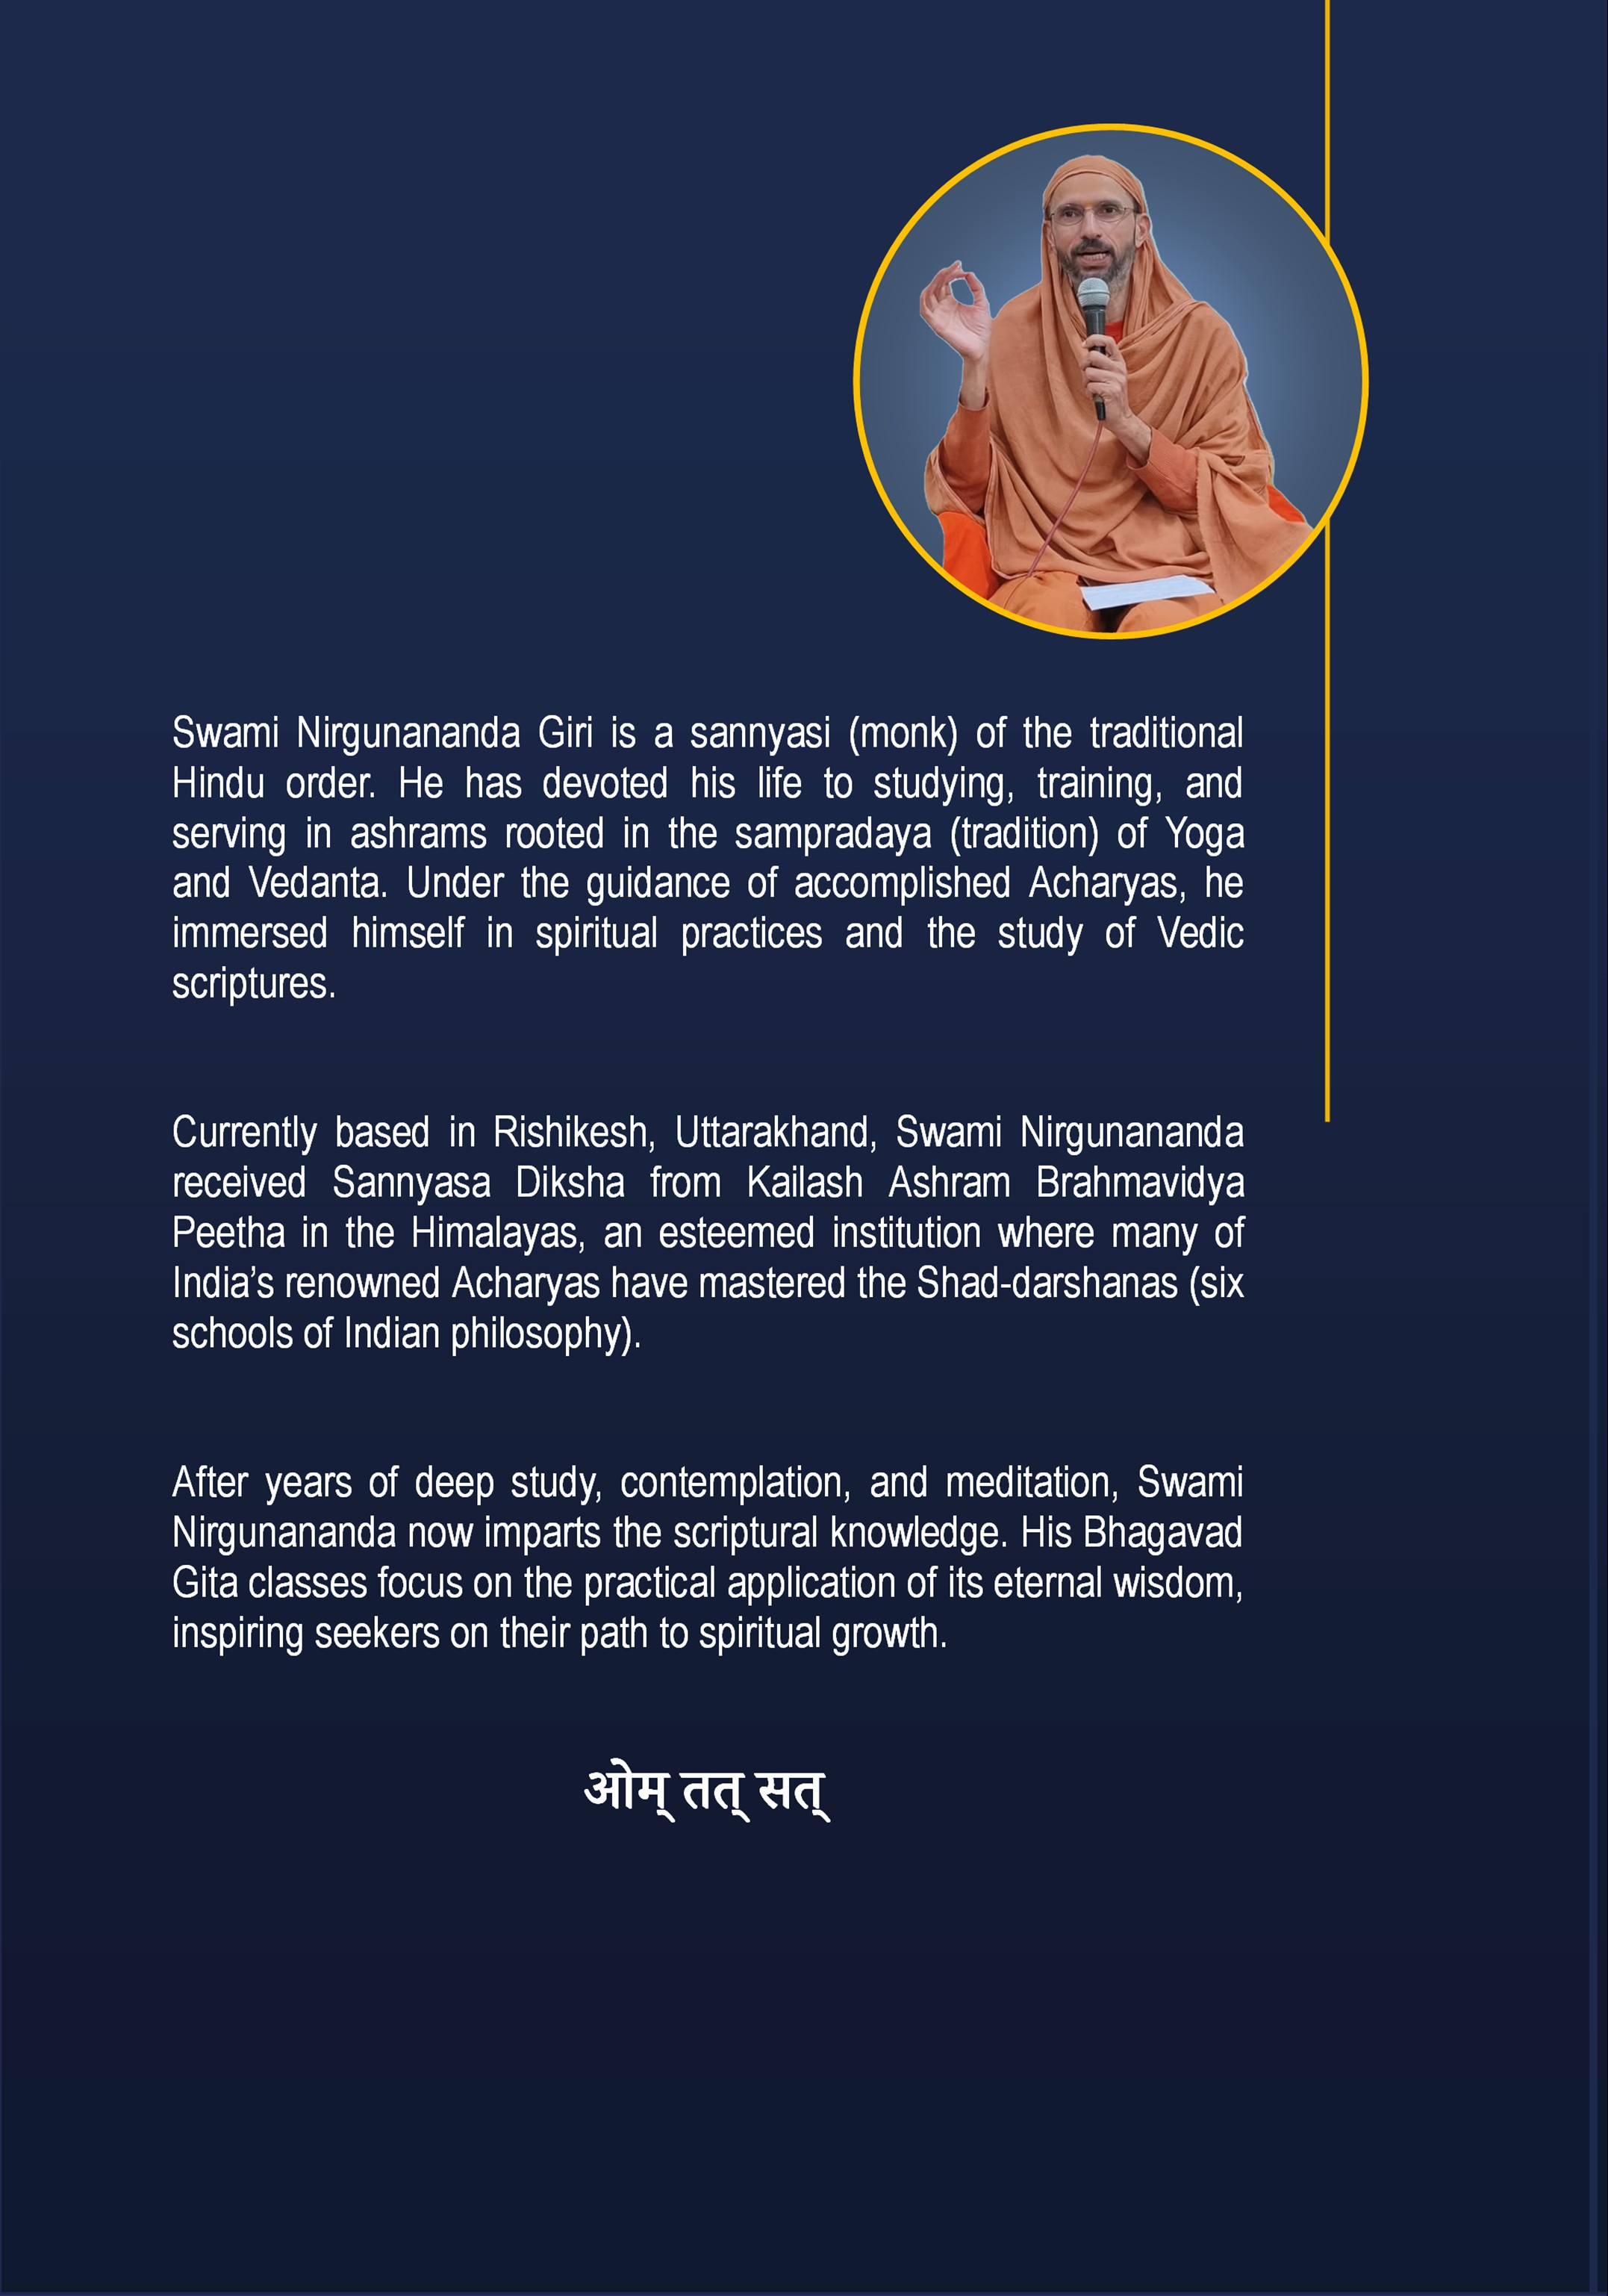
\includegraphics[width=\paperwidth,height=\paperheight]{../images/page02.jpg}%
    }%
	}
   \else% do nothing
   \AddToShipoutPictureBG*{%
    \AtPageLowerLeft{%
        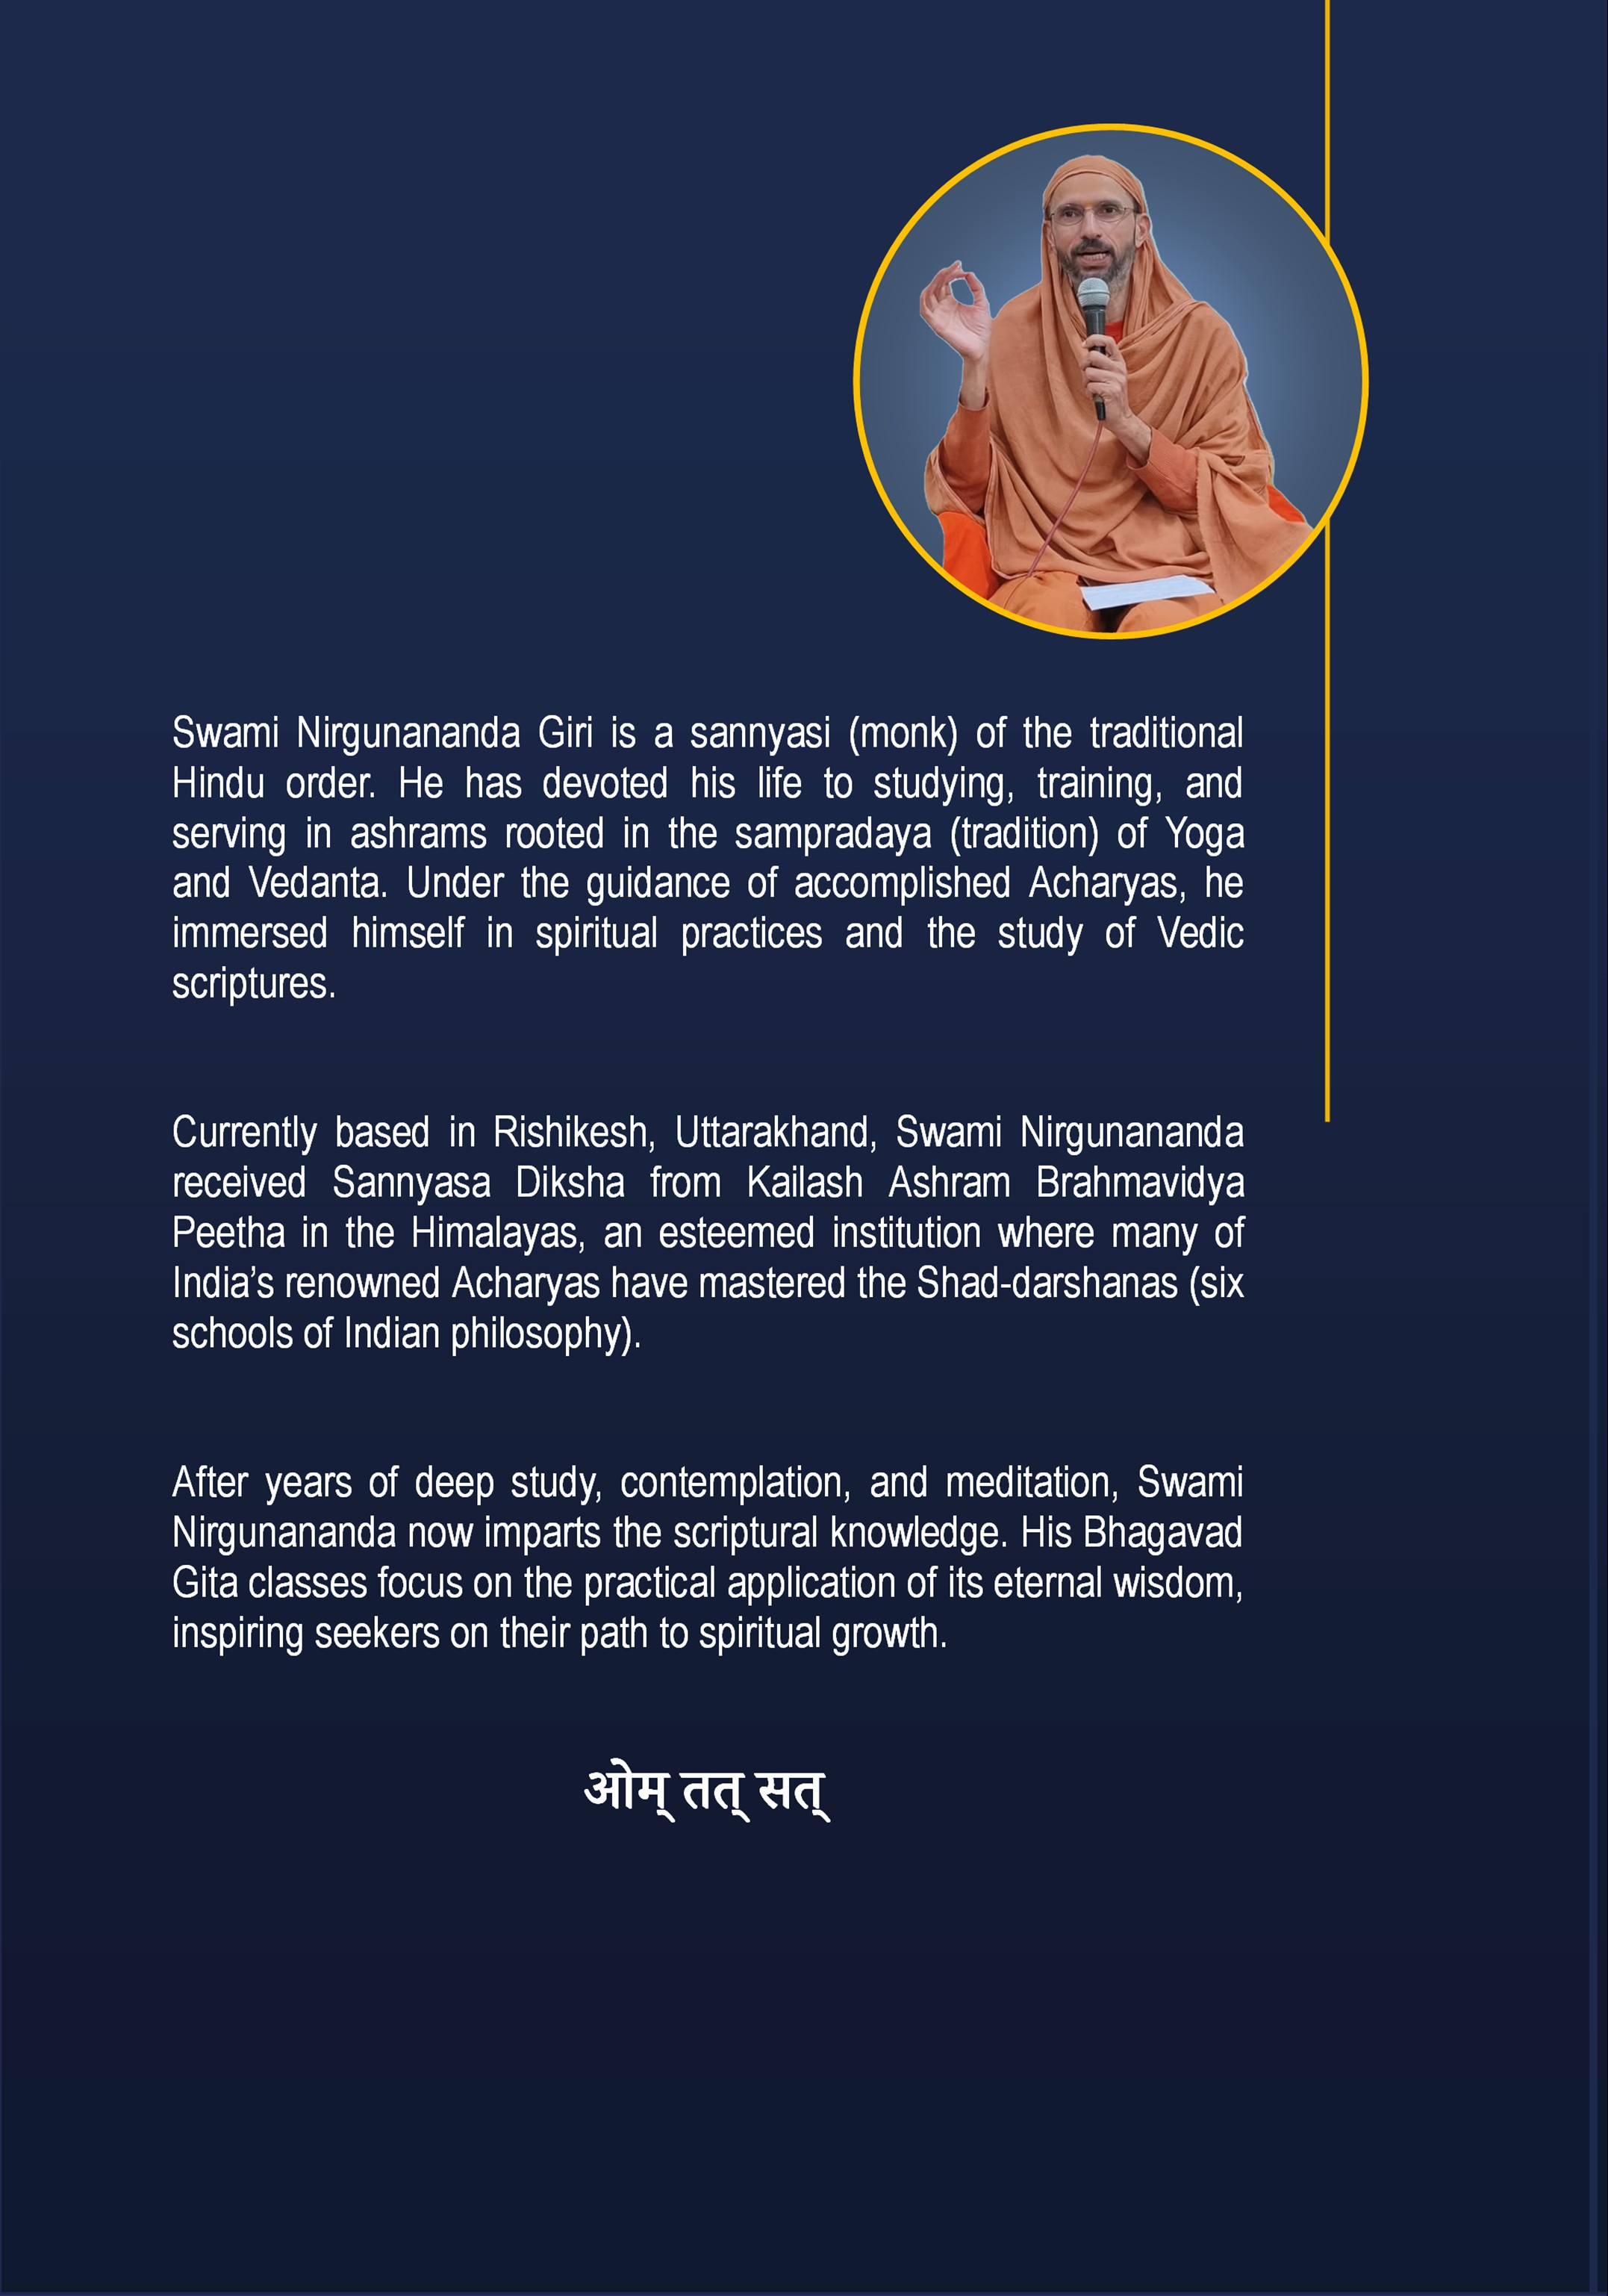
\includegraphics[width=\paperwidth,height=\paperheight]{../images/page02.jpg}%
    }%
	}
\fi
\begin{titlepage}
	%\pagecolor{pastelblue}
	\AddToShipoutPictureBG*{%
    \AtPageLowerLeft{%
        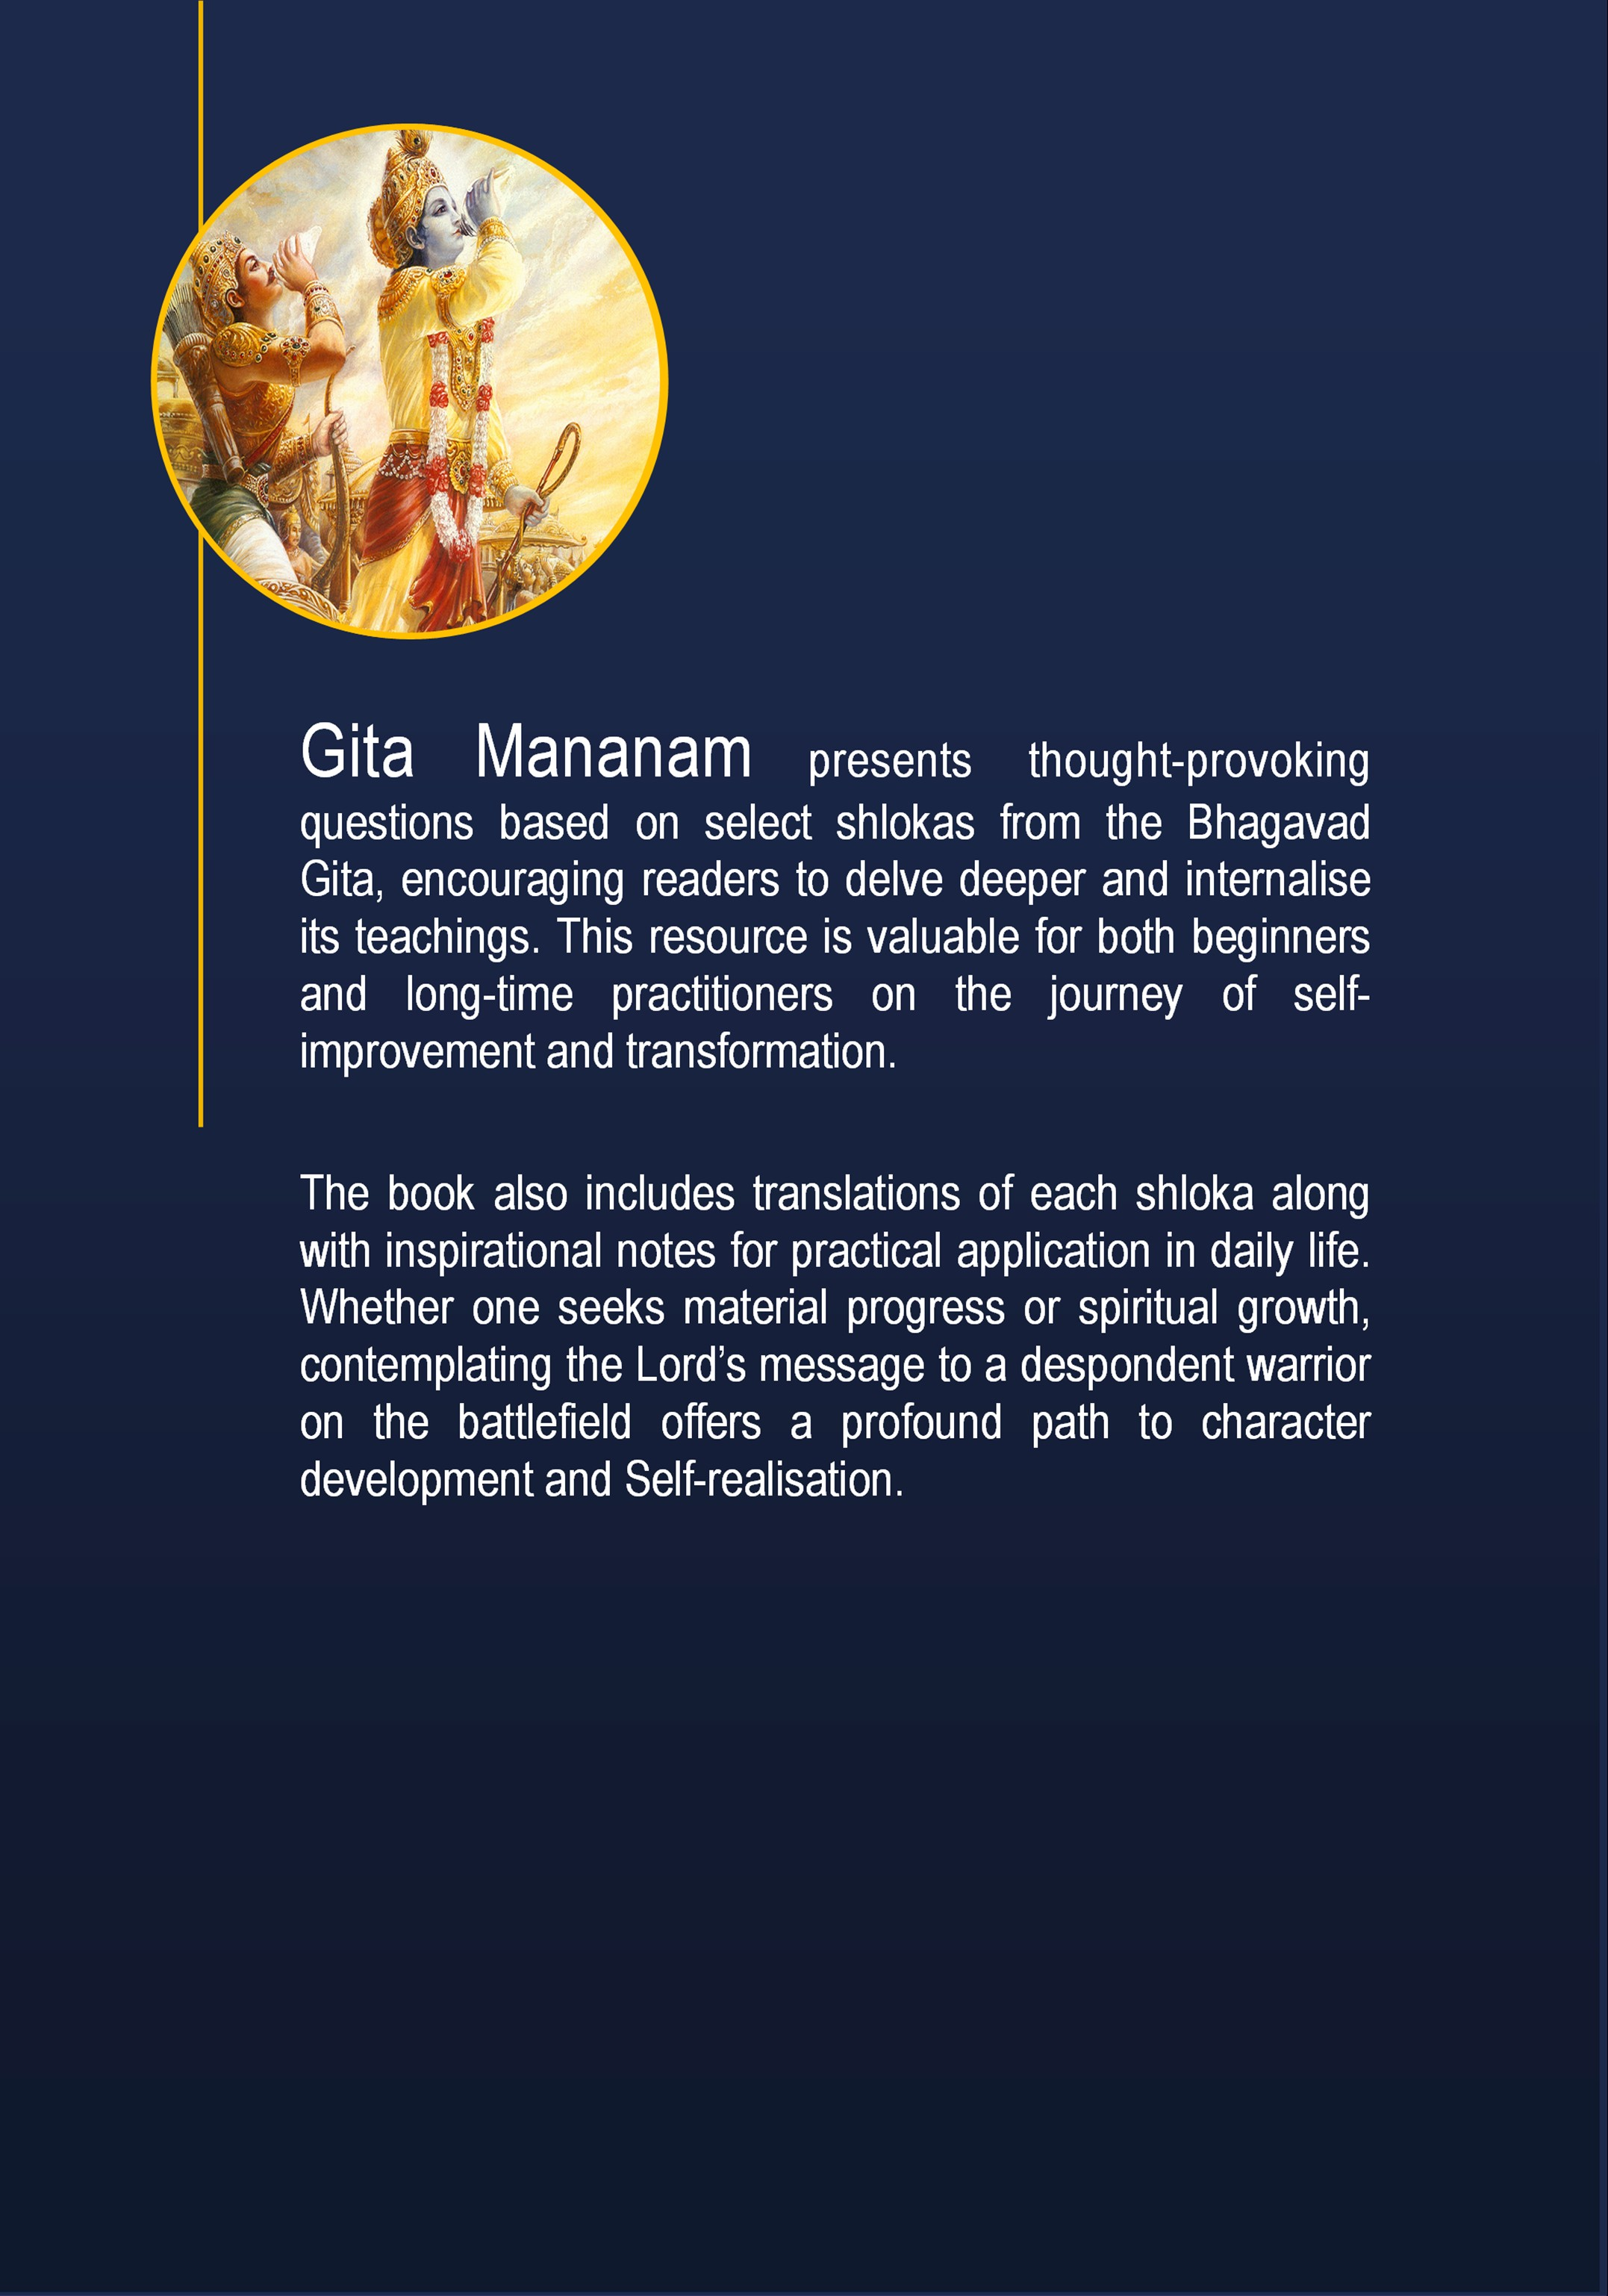
\includegraphics[width=\paperwidth,height=\paperheight]{../images/page03.jpg}%
    }%
}
    \begin{center}
        \vspace*{0.5cm}
            
        {\Huge
        %\textbf{\color{white}\fontsize{50}{60}\selectfont ಗೀತಾ ಮನನಂ}
		}
        %\textbf{\\ \small \color{white}ದೈನಂದಿನ ಸ್ಪೂರ್ತಿ ಹಾಗೂ ಆತ್ಮಾವಲೋಕನಕ್ಕಾಗಿ}    
        \vspace{1.0cm}
            
        
		
            
        \vfill
            
        
            
        \vspace{0.1cm}
        {\color{white}    
		%\textbf{{\Large \mananamfont ಸ್ವಾಮಿ ನಿರ್ಗುಣಾನಂದ ಗಿರಿ}}\\
		%{\normalsize Swami Nirgunananda Giri\\Rishikesh, India}
        }
    \end{center}
\end{titlepage}
\nopagecolor% Use this to restore the color pages to white
\end{document}
